\chapter{Mosaicing Scenes with  Vacant Spaces}
\label{ch:vacantSpaces}
\section{Introduction}
Finding features and using them to align images to construct wide
field of view panoramas is one of the success stories of computer
vision.  Virtually all recent consumer cameras have this technology
embedded.  The success of these methods relies significantly on
finding common features in the images that can be used to establish
the appropriate warps to register the images together.

\begin{figure}
  \centering
  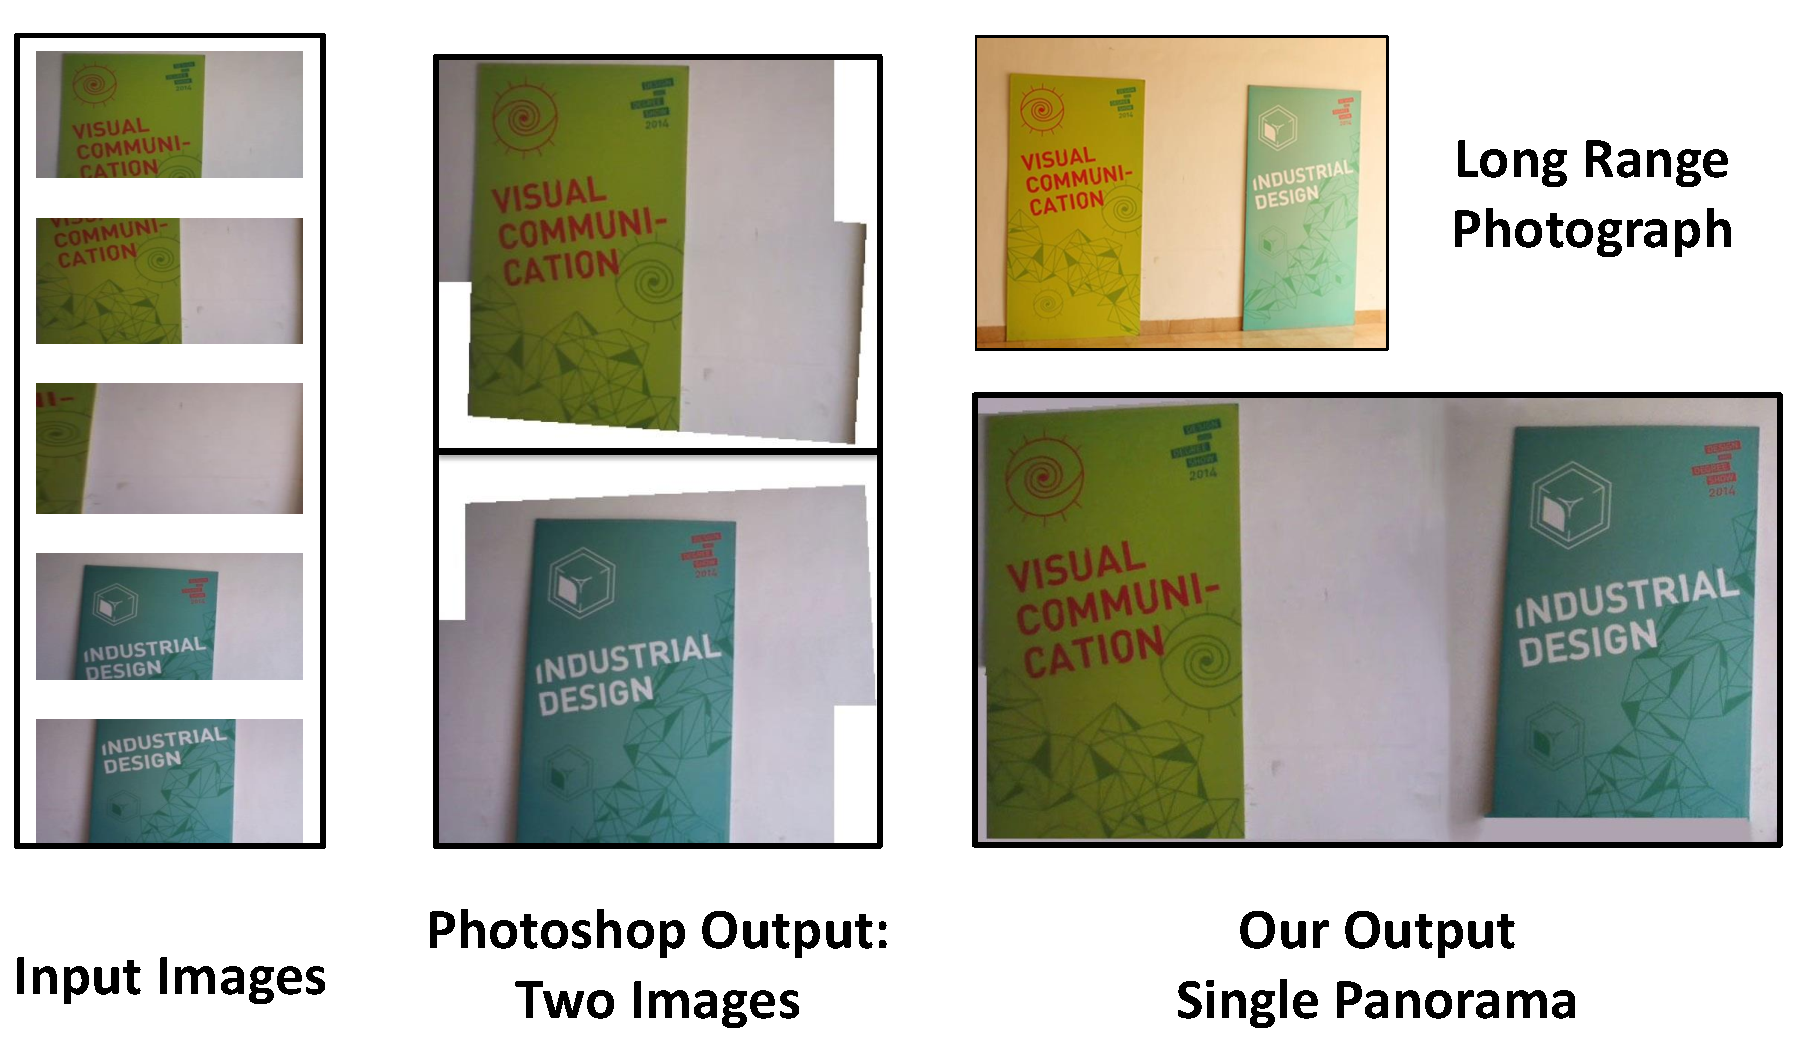
\includegraphics[width=0.8\textwidth]{figures/vacantSpaces/teaser.pdf}
  \caption[Overview]{ \label{fig:vacantTeaser} The long range photograph of a scene
    taken from an SLR camera is shown in top right.  When such a scene
    is probed by a quadcopter, it results in the input images shown on
    the left (color balance is different from the SLR camera).  The
    state of the art methods (middle column) are unable to make a
    \emph{single} mosaic because the vacant space (third picture on
    the left) does not seem to have any matchable features with
    subsequent input images. Our method handles this situation (bottom
    right).  }
\end{figure}

There are scenes, however, that consist of image content that makes
this challenging.  One situation is when the scene needs to be probed
in an orthographic view, and is not easily accessible.  Murals on
urban architecture is an example. Another situation is when scene
patterns and texture are repeated (too many similar features in, e.g.,
an outdoor art exhibition).  This can make it challenging for a
matching algorithm to find appropriate matches in large panoramas.  A
related situation is when a scene area simply does not contain
features (too little, or no features, e.g. posters in an event).
Fig~\ref{fig:vacantTeaser} shows an example of this case.  The state of the
art methods are unsatisfactory.  The idea of a moving quadcopter
taking pictures suggests using a Structure from Motion (SfM) paradigm.
However, based on our experiments with Bundler\cite{Snavely06,
  Snavely07} and VisualSFM \cite{Wu13}, we see that the success of SfM
depends very strongly on ``good'' correspondences between input
images, absent in large vacant (featureless) spaces. Specialized -- state of the art -- image stitching 
methods from \cite{Brown03, Brown05} used in tuned software like Adobe 
Photoshop CS6 or AutoStitch \emph{also} do not work as can be seen 
in Figure~\ref{fig:vacantTeaser}.


The goal in this work is to create panoramic images of scenes using a
quadcopter in situations described above. From a vision perspective,
we are excited about a new mosaicing problem containing large
homogeneous vacant spaces.  This results in scene regions that have no
matches between many significant images, and therefore cannot be
aligned using traditional mosaicing methods.


{\bf Key Idea} We propose to solve the vacant space problem by using
an inexpensive off-the-shelf flying device, such as a quadcopter which
can be assumed to contain an inertial measurement unit (IMU) that has
positional information.  The proximity relationship that the resultant
images have, can be used to significantly reduce the search space in
finding matches.  Further, the proximity relationship also allows, in
principle, to vary the parameters involved in feature selection. For
example, if there is reason to believe that two images are adjacent
horizontally, one can choose to adjust thresholds in feature matching
algorithm to hunt for otherwise elusive matching pairs.

We note that IMU data can be also made available in other devices such
as smartphones.  An autonomous programmed quadcopter, however, is
particularly enticing because of its ability to fly to areas that are
accessible to the human eye, but inaccessible for the human to
reach. Such areas do not lend themselves easily to high quality
images. 

Further, IMU data, whether on a smartphone or on a quadcopter, cannot
be relied exclusively, or sometimes at all, especially on inexpensive
devices. Our experiments indicate that the roll and pitch angles
(depending on the distances involved) may be completely off, and so
can the physical coordinates.  This is a consequence of the jerky,
swift movements.  Complementing the IMU with information gleaned from
vision algorithms, however, may be a useful practice.

{\bf Contributions} The main technical contribution of this work is
that it improves the state of the art in mosaicing.  We assume that
the imagery is acquired by a quadcopter for the reasons mentioned
above. Sending a battery of images from a quadcopter to an image
mosaicing algorithm such as AutoStitch incapacitates the algorithm
because of the sheer number of images. Sending a sampled version of
images to a manageable number $N$ of images, with $O(N^2)$ possible
areas to match for features, also does not work since the sampled
image contains vacant space.  In this work, we use IMU information
that lends itself to a graceful $O(N)$ algorithm.  Results are
available in the experiments section. In summary we have a solution to a new problem, and a
faster solution using IMU data.

%{\bf Limitations} 
In this work, we assume that the scene lies on a planar surface, or
approximately planar surface. The quadcopter can also be programmed to
have a viewing angle perpendicular to any desired planar structure.
The standard homography computation is still not possible because of
the vacant spaces. To overcome this, we reduce the mosaicing problem
to the stereo problem and are thus able to complete the panorama.

% The rest of this paper is organized as follows.  In the next section,
% we discuss related work.  Subsequently we describe the main steps in
% our process, and justify the process in Section~\ref{sec:results} with
% experimental results. (Additional results are available in
% supplementary material.)  The final section discusses future work.

\section{Methodology}

The goal of this work is to compute a panorama of a scene lying on
planar surface that has regions of vacant spaces.  A schematic for
this problem is shown in Figure~\ref{fig:schematic}. 

\begin{figure}[h!]
  \centering
  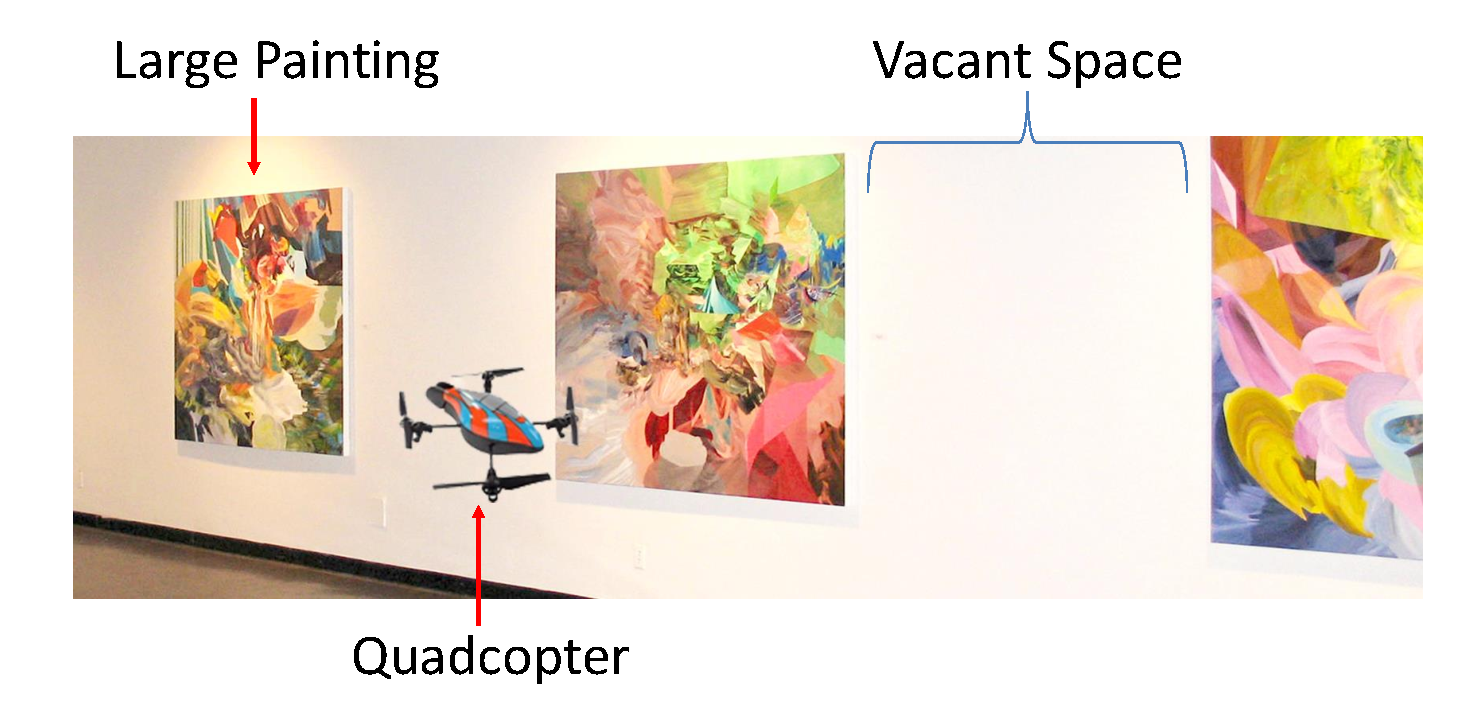
\includegraphics[width=0.8\textwidth]{figures/vacantSpaces/indoor}\\
  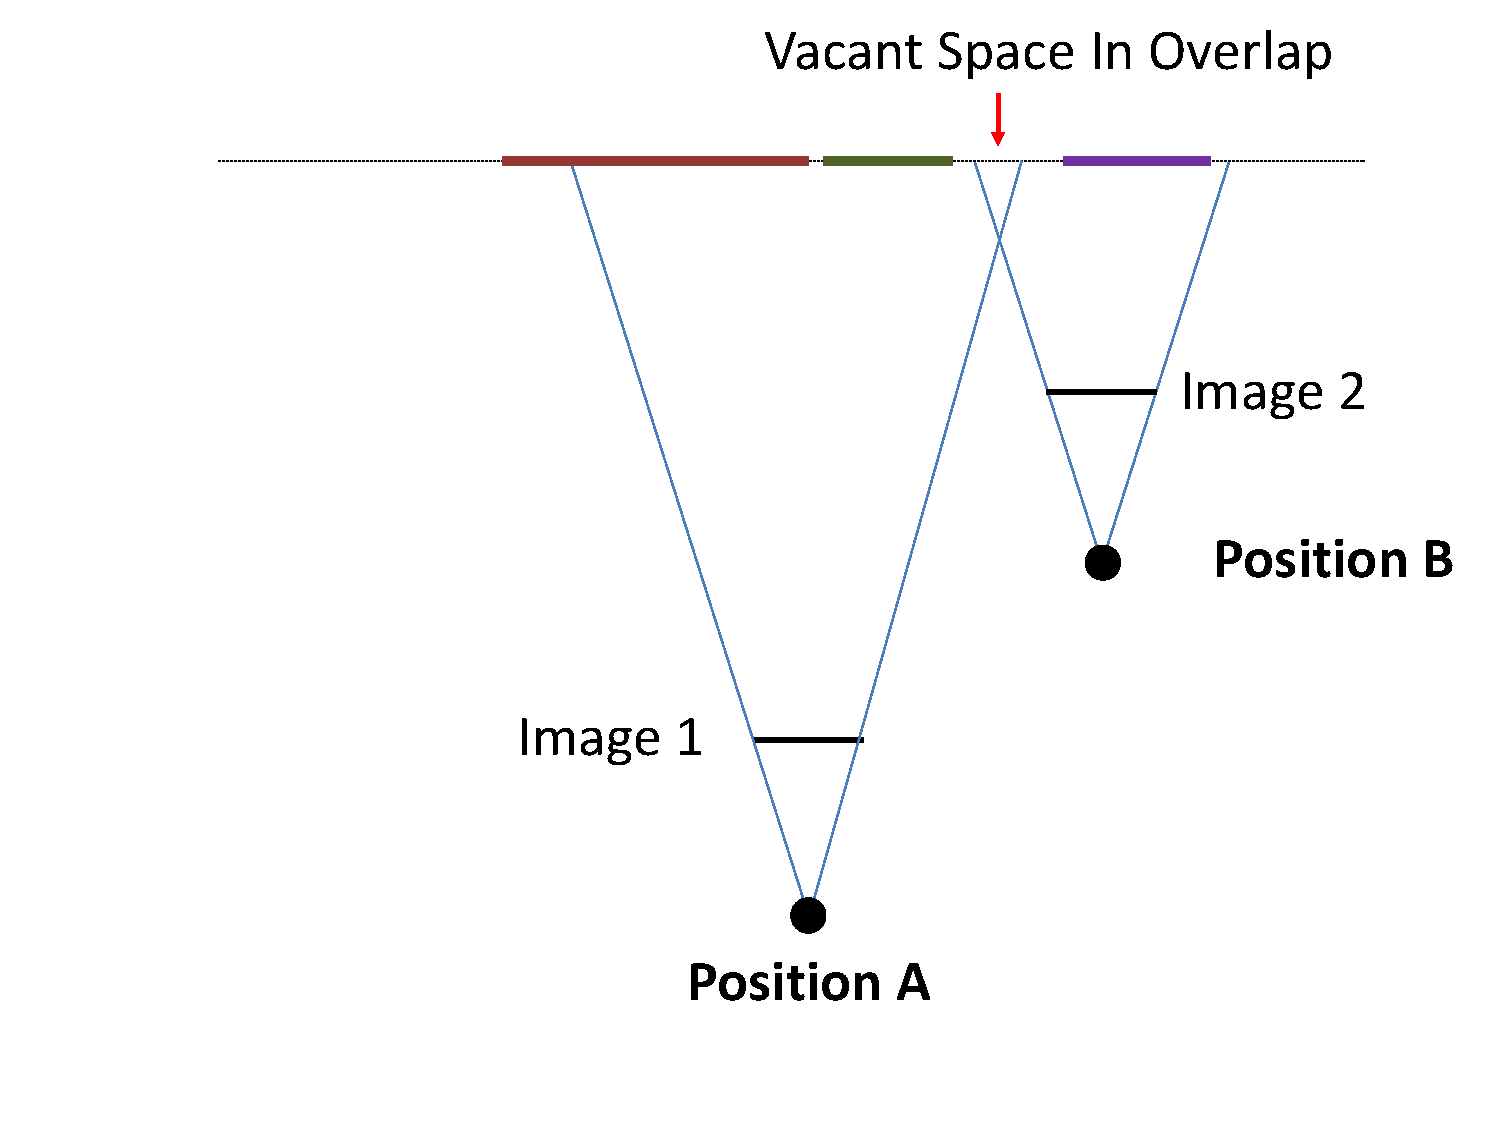
\includegraphics[width=0.8\textwidth]{figures/vacantSpaces/stereoOverlap}\\

  \caption[Problem definition]{ \label{fig:schematic} Problem definition. (Top)
  Vacant spaces are encountered in various scenes.  When individual portions are
    captured by a quadcopter, how does one create the complete mosaic
    given that common features are either not available, or
    confusing? (Bottom) Simplified reduction of the problem to a geometrical structure.
  }
\end{figure}    

The method adopted is pictorially depicted in the overview shown in
Figure~\ref{fig:vacantworkflow} and is described in detail later on.  In
brief, we systematically acquire a video of the scene, reduce the
input video to a manageable number of images, and finally combine the
images acquired from different positions into a mosaic.

\begin{figure}[h!]
  \centering
  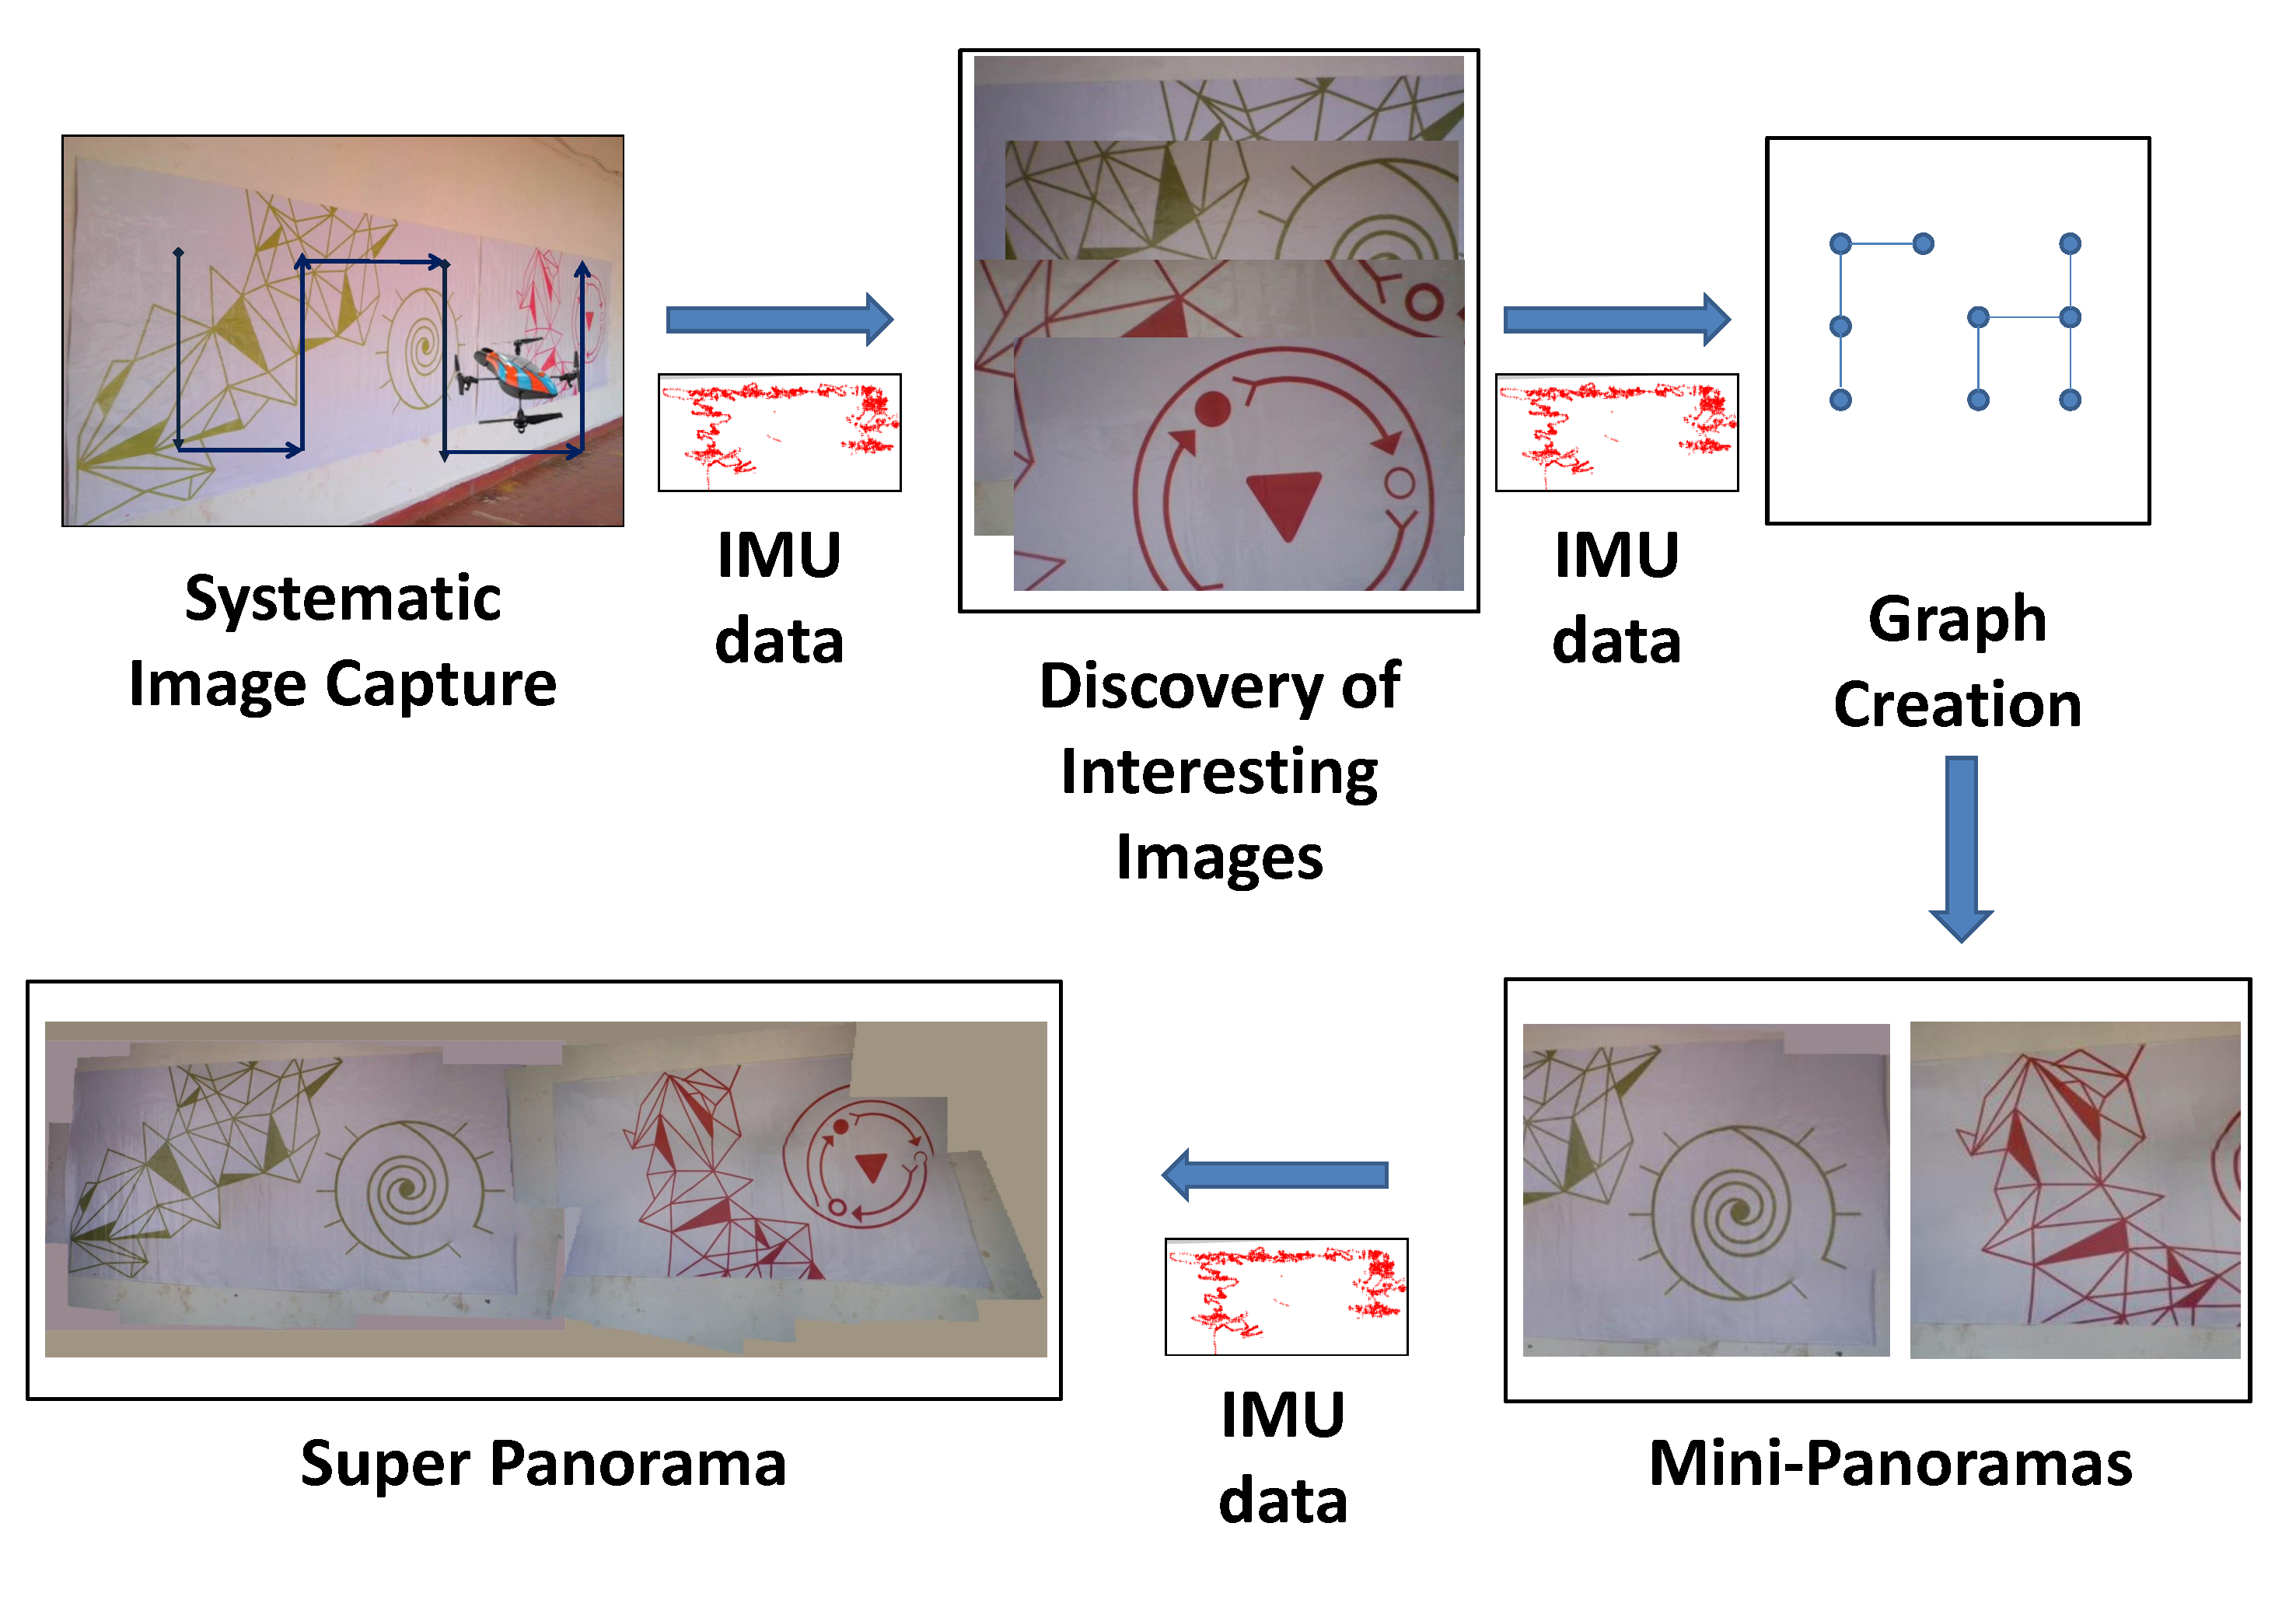
\includegraphics[width=\textwidth]{figures/vacantSpaces/Workflow} 
  \caption[Workflow]{ \label{fig:vacantworkflow} Overview: Input imagery is
    systematically acquired (top left) by a quadcopter.  In the next
    step, interesting images are found by clustering the video into
    regions based on positional data.  A graph is constructed using
    proximal images. For each connected component in a graph, standard
    stitching techniques are used to create mini-panoramas which are
    then joined together into super panorama 
    again using IMU data.}
\end{figure}    


\subsection{Video acquisition}
We first dispatch the quadcopter to as close to the scene as
possible. The corners of a rectangular area of interest are provided
to the quadcopter, and it is programmed to traverse the area in a
raster scan fashion.  There are various control aspects involved in
sending a quadcopter; in outdoor areas, the quadcopter is impacted by
wind and it might lose its way.  The control aspects of the quadcopter
is beyond the scope of this work.  \emph{Note that trying to create a
  mosaic in an incremental linear fashion by combining adjacent frames is
  prone to loss of two-dimensional spatial proximal information. It is also
  computationally overwhelming.}

The quadcopter returns with a video of the scene.  Images extracted
from a short video of about a minute or more overwhelms existing
mosaicing software, such as AutoStitch or Adobe Photoshop.  In the
rest of this section, we use AutoStitch to indicate state of the art
stitching programs such as AutoStitch, Photoshop, etc.

\subsection{Acquiring interesting images}
\label{sec:selection}
Our goal in this step is to reduce the amount of input data and
produce a set of interesting images.  In other words, we wish to
convert a video into an album of images.  The key difference between
our problem and standard albumization \cite{Aner, Lee} is the use of
positional information.  A standard quadcopter has an inertial
measurement unit (IMU) that, after calibration, may give reasonably
accurate information of positions. Using positional information it is
possible to cluster the images, and sort the images into an $m\times
n$ grid.  The number of cluster centers is automatically determined
using the agglomerative bottom up hierarchical clustering method
\cite{Lior}, with the additional requirement that the whole scene
(represented by the positional data) is covered.

{\bf Clustering Details} We assume that each IMU data position
corresponds to an image of definite fixed dimensions.  Consider each
position of the IMU data to be a leaf node. Two nodes are greedily
combined based on the closest Euclidean distance, and replaced with an
internal node; the position of the internal node is set to be the
centroid of the two nodes, and each internal node now corresponds to a
virtual image of the same size taken by a virtual quadcopter.  The
algorithm recursively merges all the nodes till we end up with a root.
In the next phase, we produce cluster centers; a set of nodes is
considered for being the output as cluster centers if the union of
these nodes completely cover the scene. From the bottom-up
construction, it is clear that the root will represent a single
position, and thus a single virtual image, and will not cover the
scene.  At the other extreme, the set of all leaf nodes \emph{will}
cover the scene. To resolve this, during the calibration phase, we
pre-decide the minimum distance between two center of projection to
have least overlap. This is used as the threshold in the clustering
algorithm.  Once cluster centers are found, we pick the leaf node
which is closest to the cluster center to find a real image. This
process is schematically shown in Figure~\ref{fig:selection}.

If we had no IMU information, one may consider selecting a
set of interesting images using any appearance based method such as
optical flow or feature selection.  However, due to the jerky and
uneven motion of the quadcopter, such measures do not prove to be
sufficient. On the other hand, on inexpensive quadcopters, we have
encountered several cases of erroneous positional information (we note
here that image computations are not on-board the quadcopter and IMU
information is transmitted via WiFi to a host computer).  

% We believe
% that combination of standard vision-based clustering method with the
% clustering based on positional information can be used to either drop
% frames, or to correctly include frames based on image content.

\begin{figure}[t!]
  \centering
  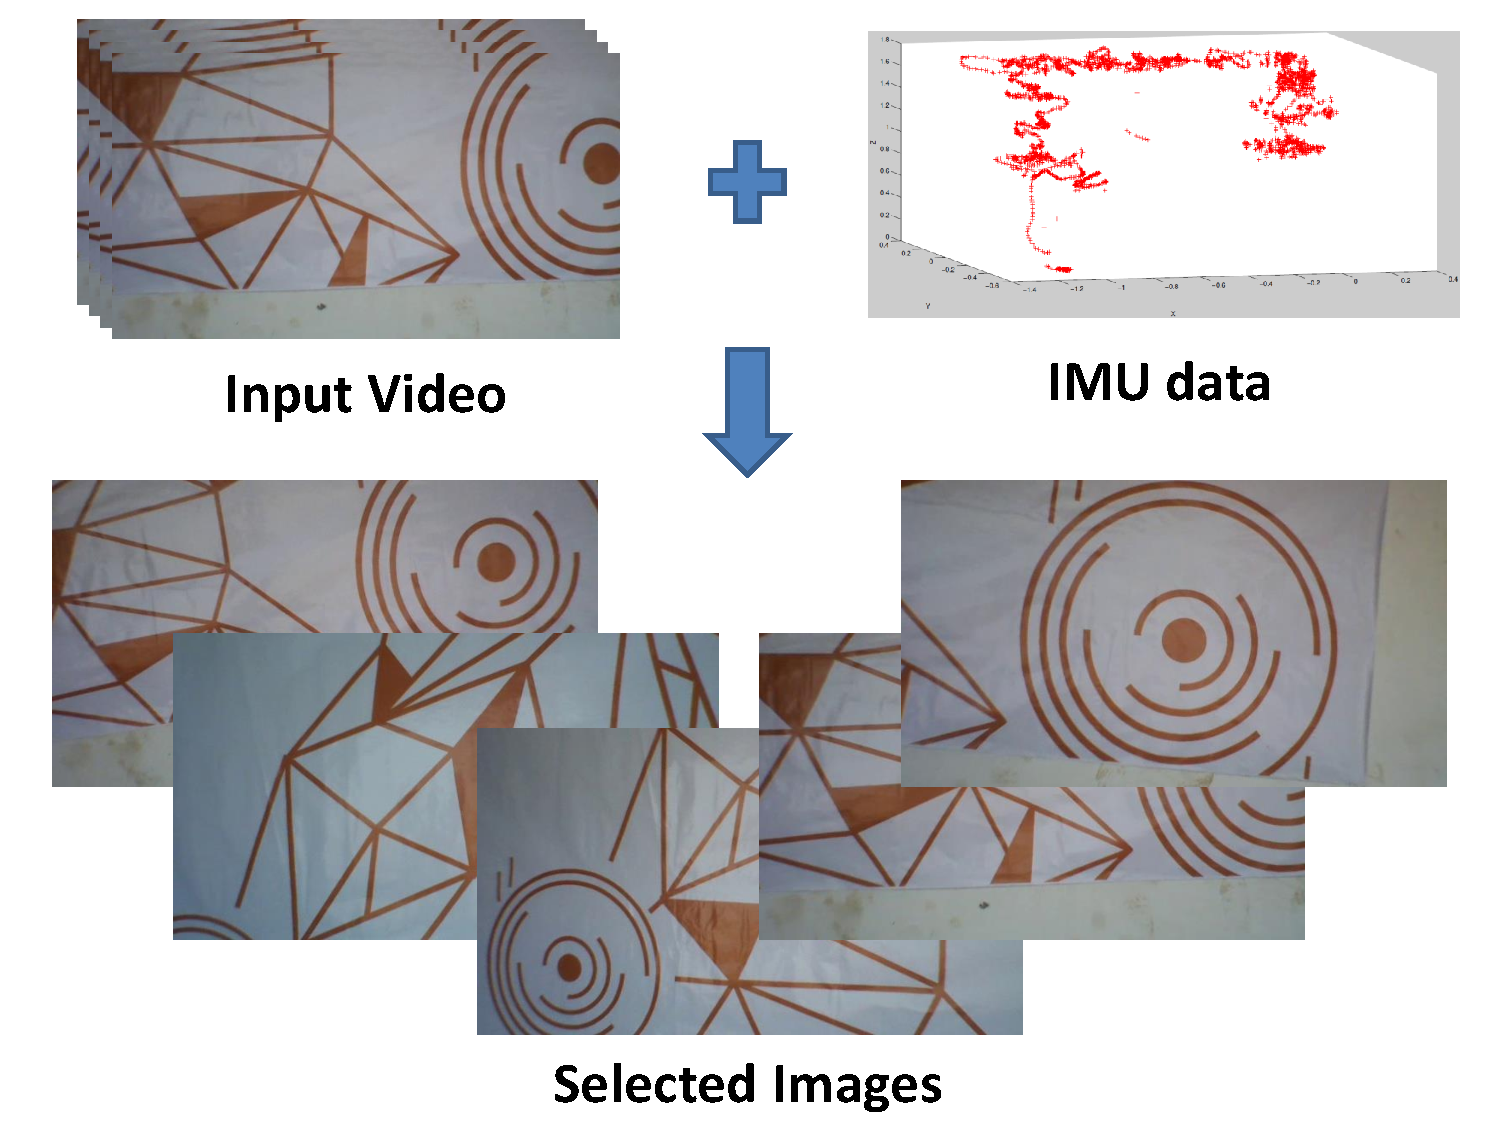
\includegraphics[width=0.42\textwidth]{figures/vacantSpaces/selection} 
  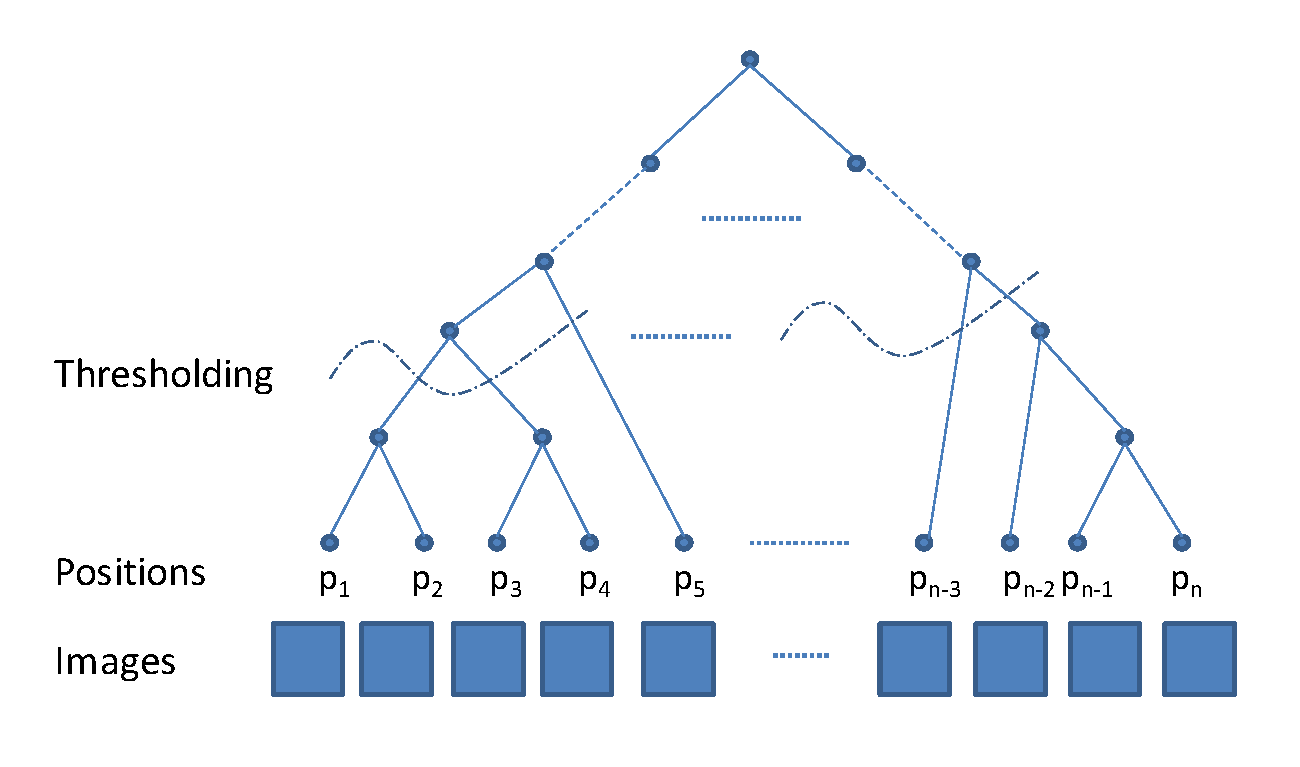
\includegraphics[width=0.56\textwidth]{figures/vacantSpaces/clustering}
  \caption[Selection of Images]{ \label{fig:selection} Left:We align the image
  stream with IMU data, and then transform the video into a set of interesting
    images with a clustering algorithm. Right: Hierarchical clustering is done
    on the positional data to find out the optimal number of positions which
    `encompasses' the scene. Threshold based on the average distance of the
    quadcopter from the plane is used to prune the tree.}
\end{figure}    

In practice, the number of cluster centers for the scenes we have
covered is now within the capacity of AutoStitch.  As mentioned in the
introduction, as long as there are sufficiently varying and
``matchable'' features, AutoStitch is able to perform a reasonable
result.  However, if there are very few features in overlapping region
of two images, then the output is not acceptable. This situation will
arise when there is vacant space between two pictures.

{\bf Time complexity} AutoStitch has not been designed
to use positional information. As a result if there are $N$ input
images, the program has to consider possible matches in approximately
$O(N^2)$ set of areas.  Our program is able to mosaic in an $O(N)$
fashion.

{\bf Mini-Panoramas} Specifically, we assume at this point that the
interesting photos are available in the form of a $m \times n$
grid. First, we find SURF \cite{Bay} features for each image in a
grid. Next, we use Best of Nearest Neighbor matcher (from the OpenCV
library) with Random Sample Consensus (RANSAC) \cite{Fischler1981} to
find geometrically consistent matches between neighborhood images
inside grid.  We create a graph with images being nodes, and add an
edge between two nodes if there are sufficient matches. We have to
recall at this point that if there are ``vacant spaces'' there will
not be enough features for successful matches; the graph will end up
with multiple (disconnected) components.  We next compute multiple
spanning trees for the various components. Given a spanning tree, the
center of the spanning tree is a node from which the distance to all
other nodes is minimal \cite{Kocay}. Next we calculate the homography
of each image with respect to spanning tree center.  Finally, for each
spanning tree, we stitch all pictures within the spanning tree to
create a mini-panorama using the computed homographies by warping all
images with reference to the image at spanning tree center. The
spanning tree is an $O(N)$ structure. The process is described in
Figure~\ref{fig:graph}.

\begin{figure}[t!]
  \centering
  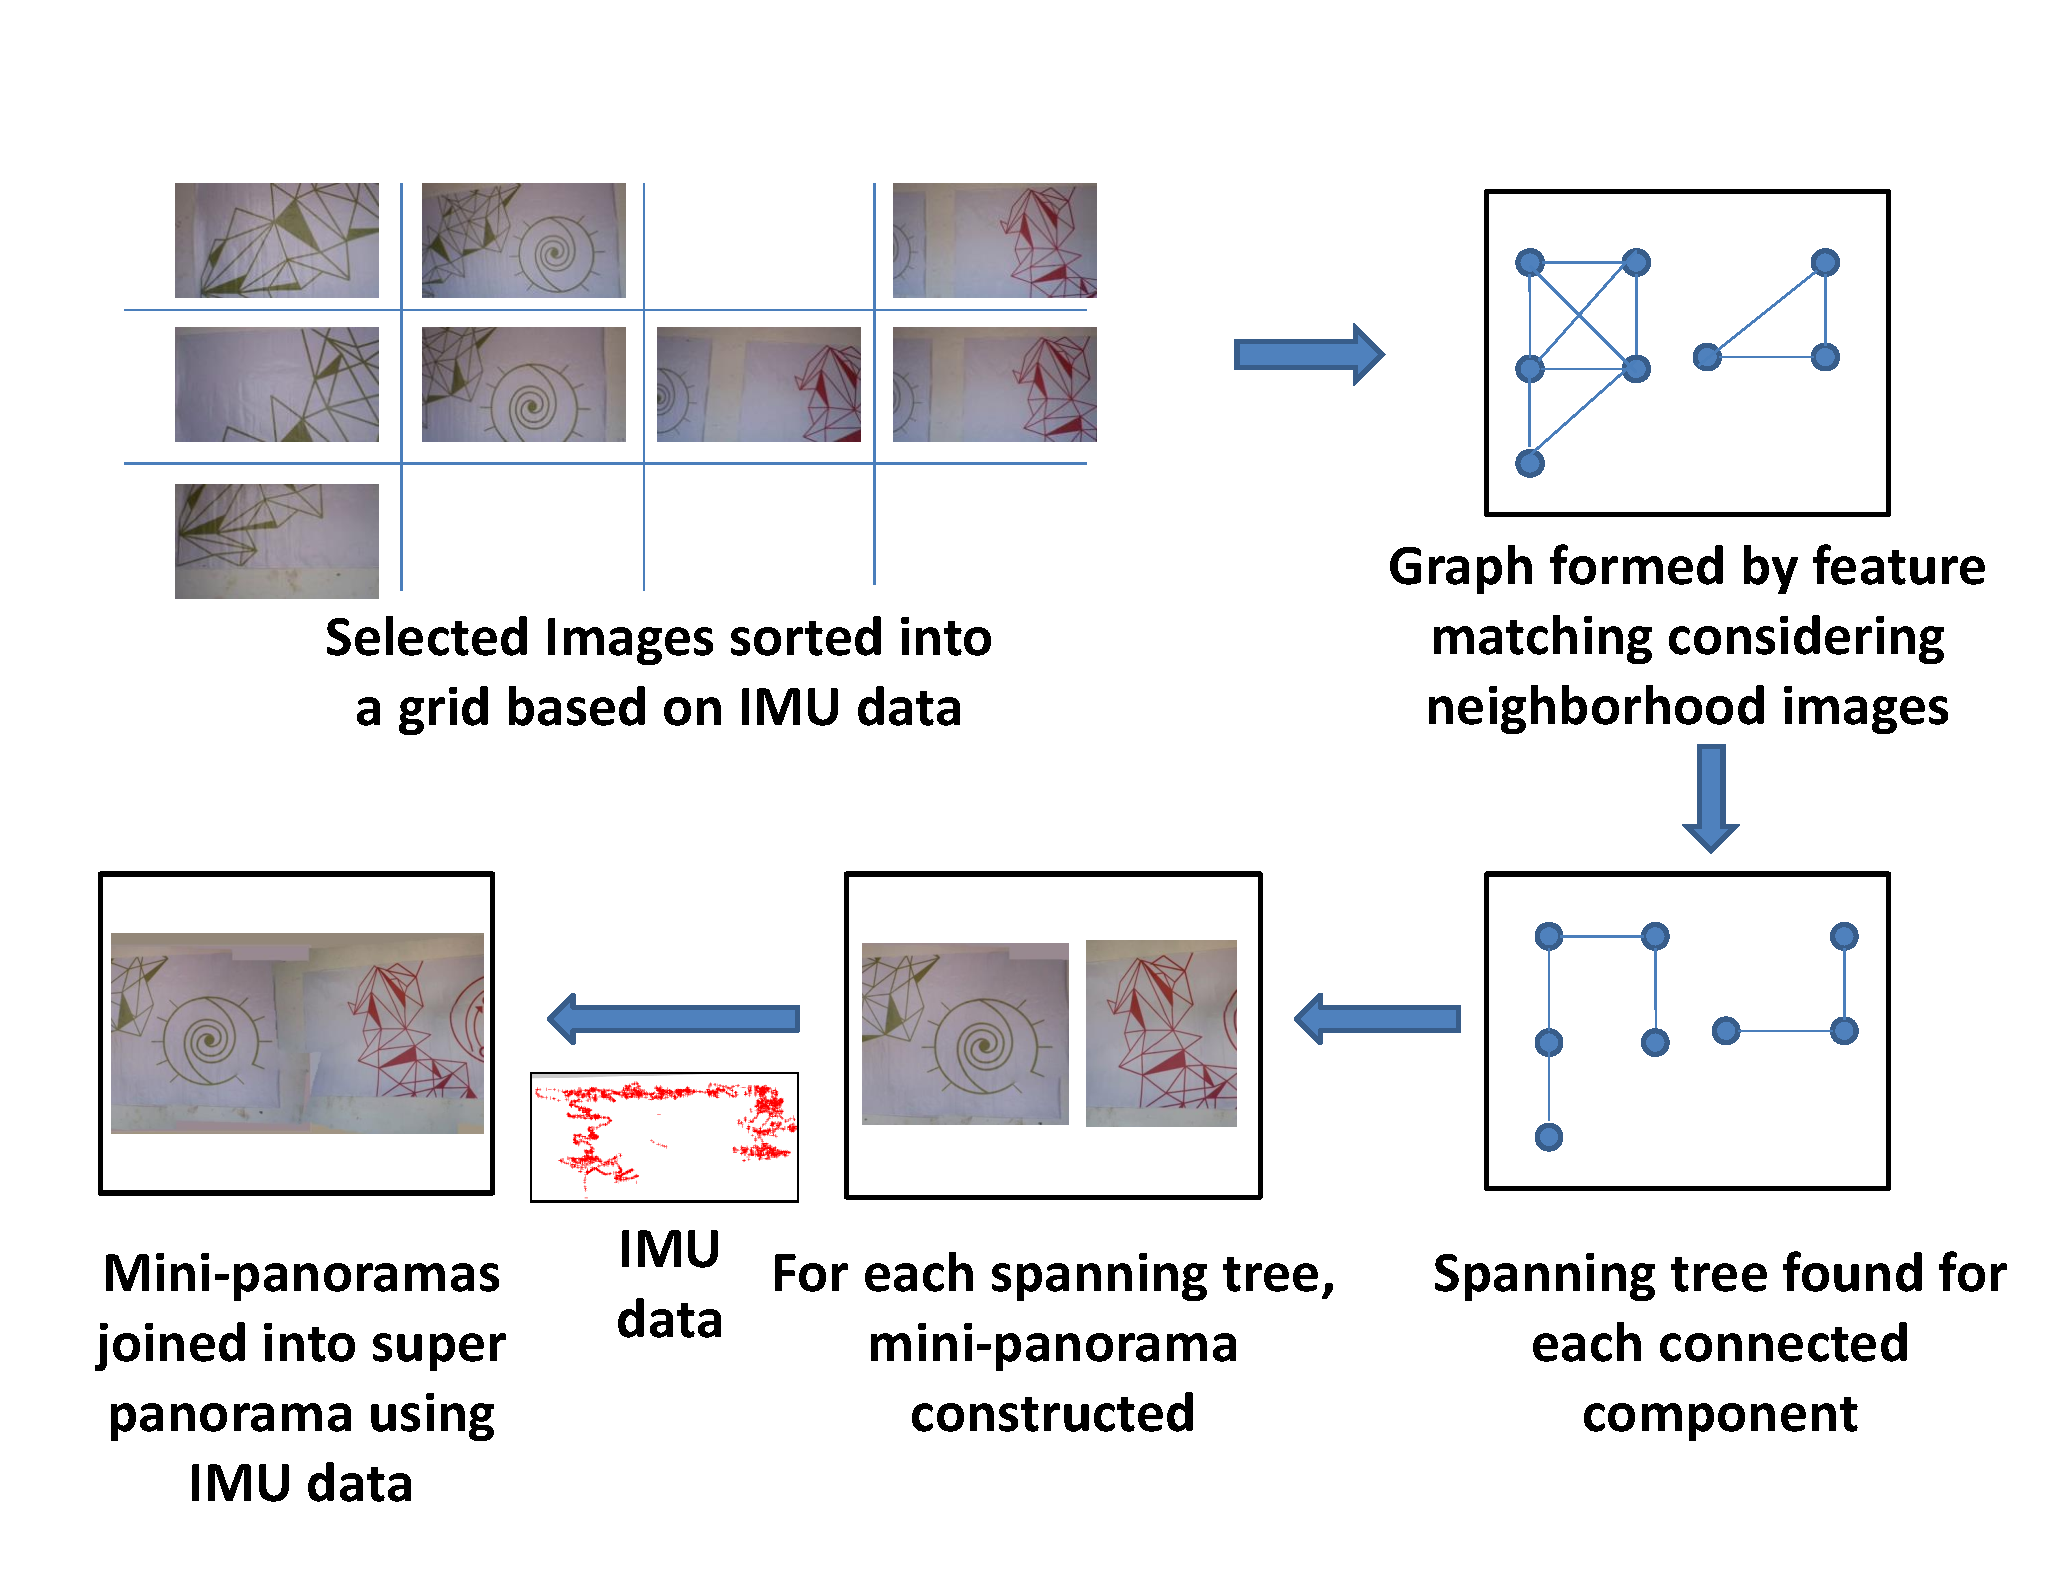
\includegraphics[width=\textwidth]{figures/vacantSpaces/graphCreation} 
  \caption[Creation of Mini-panoramas]{ \label{fig:graph} Interesting images
  acquired are segmented and individual (mini-panoramas) are constructed. These
    are then later combined into the desired super-panoramas using IMU data.}
\end{figure}    

\subsection{Super-panorama}
In this section, we consider the situation when programs like
AutoStitch fail.  We assume that the output of the previous step has
resulted in multiple spanning trees where each spanning tree center
corresponds to a specific depth . This is the depth of the center of
the spanning tree (estimated from the IMU data), since we have stitched all images by taking the
spanning tree center as a reference.  Individual panoramas for each
spanning tree termed mini-panoramas have been created. A
super-panorama must be created from mini-panoramas; these usually
correspond to different depths for at least two reasons.

First, it is invariably difficult, if not impossible, to control a
quadcopter to be at the exact depth even in indoor scenes.  The
aerodynamics and the thrust produced tends to make the quadcopter
drift.  Second, it might also be necessary to let the quadcopter probe
and come closer to the scene so as to get a ``good picture''.

A super-panorama is done using a two step process. Assume two trees in
the forest corresponding to area A and area B of the scene (see
Figure~\ref{fig:stereo}). 
\begin{figure}[h!]
  \centering
  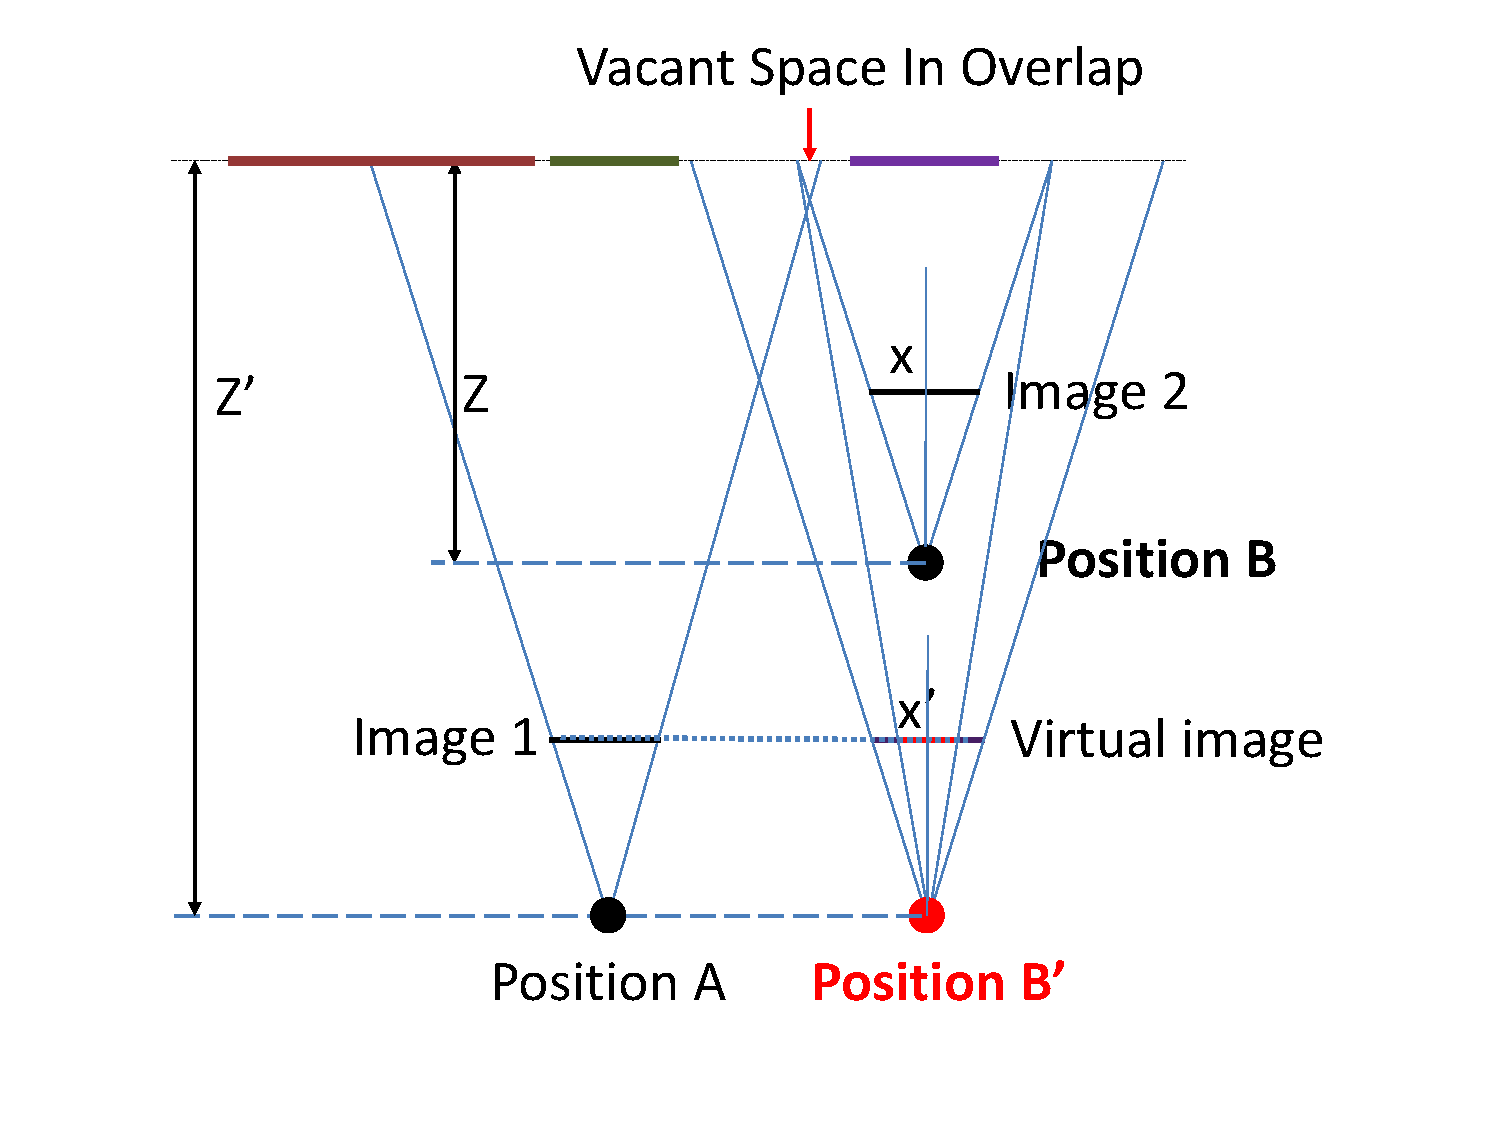
\includegraphics[width=0.8\textwidth]{figures/vacantSpaces/move} \\
  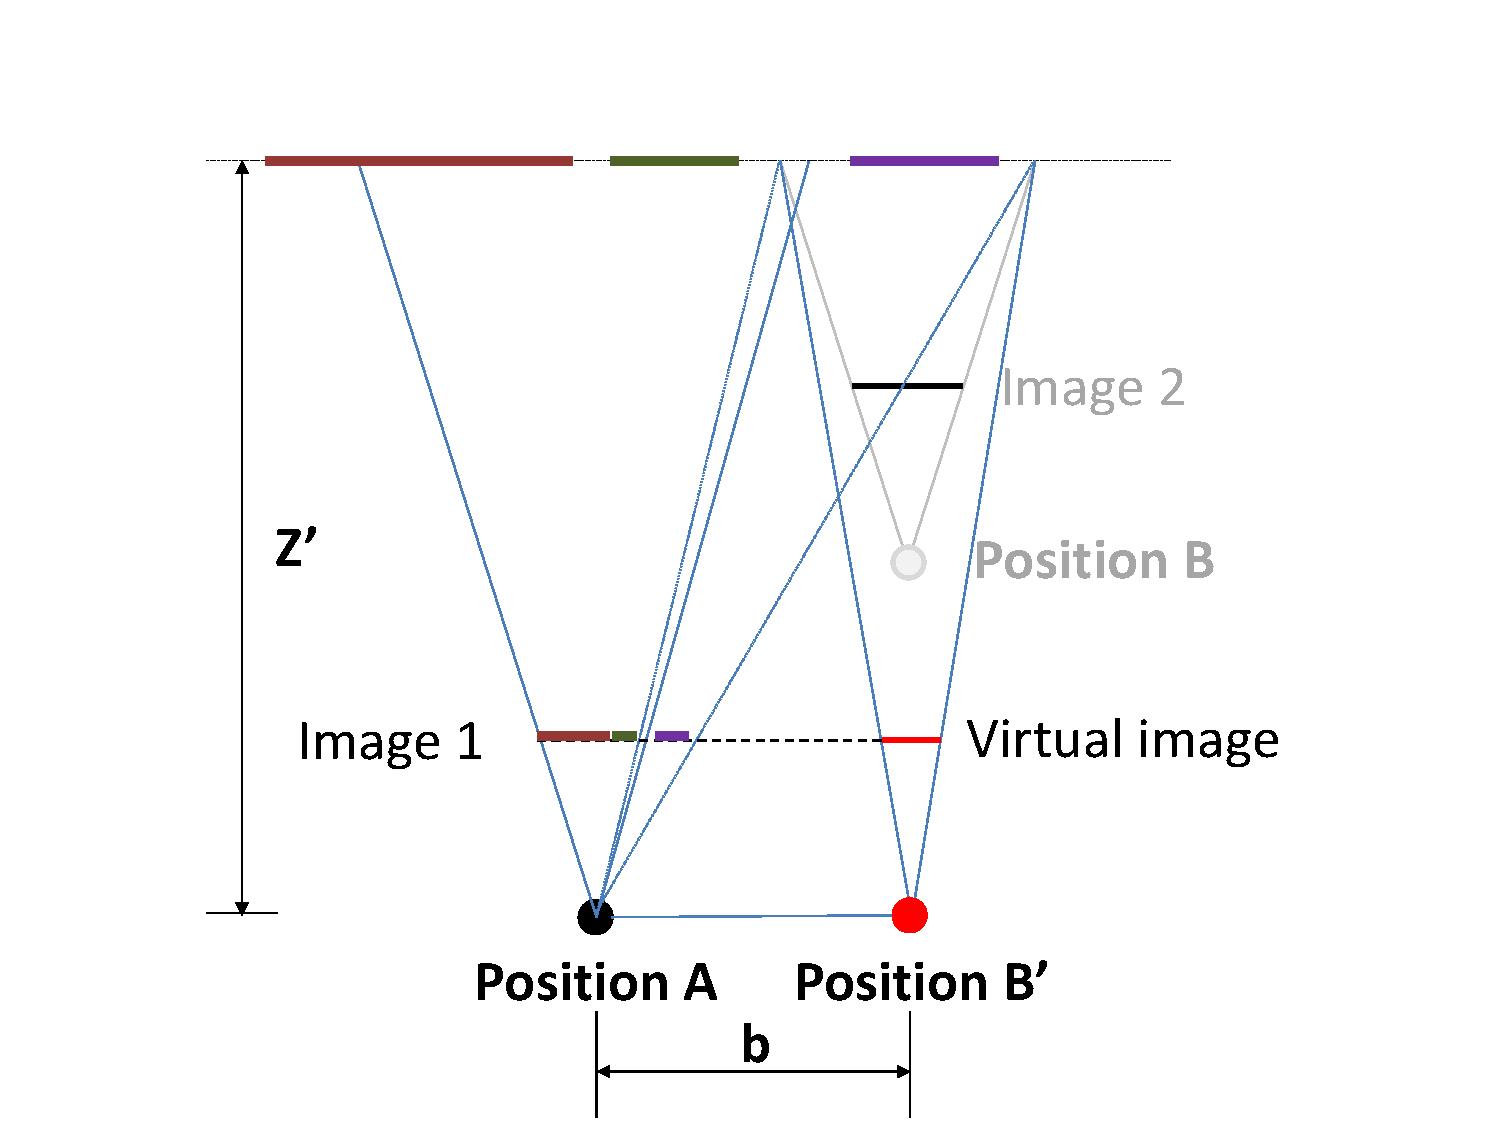
\includegraphics[width=0.8\textwidth]{figures/vacantSpaces/stereo} 
  \caption[Creation of Super-panoramas]{ \label{fig:stereo} (Top) The virtual
  picture as seen from position B' is computed using Equation~\ref{eq:moveRelation} from the real picture
    taken from B.  (Bottom) Using the stereo disparity, calculated from the baseline 
   width b and depth Z',  it is possible to depict the composite scene obtained from both A
  and B' (from the view point of A).}
\end{figure}    
Assume that a mini-panorama is created from these two areas, and the
depth of the planar surface from the camera is more for A, than for
B. We then take the mini-panorama image captured at B, and `move' it to
a new location B' whose depth (from the imaged surface) is the same as
that of A. The resulting image  will be smaller; the images are
related by the equation
\begin{equation}
  \label{eq:moveRelation}
  {\bf \frac{x'}{x} = \frac{Z}{Z'}}
\end{equation}
where {\bf x} (respectively {\bf x'}) represents a pixel location of
the image in B (respectively, B') and 
{\bf Z} (respectively {\bf Z'}) represents the depth of the images
surface from B (respectively, B').

In order to form a super-panorama from the depth of A, we can now
treat the resulting images from A (unchanged) and B’ (computed from
Equation~\ref{eq:moveRelation}) forming a simplistic stereo pair at
the depth of position A.  Using the stereo disparity formula we can
``place,'' from the view point of A, the image captured from B',
thereby creating a super-panorama. (We could as well present the
entire scene from the viewpoint of B' (since it is at the same depth);
we prefer these pictures to the one that one may be created from the
depth of B.)

% In theory, one may for the super-panorama from viewpoint B, by first
% moving position A to the same depth as of position B. But in that
% case, virtual image of A formed at the depth of position A will be
% ``zoomed-in'' version which may cause pixelization.

\begin{figure}[h]
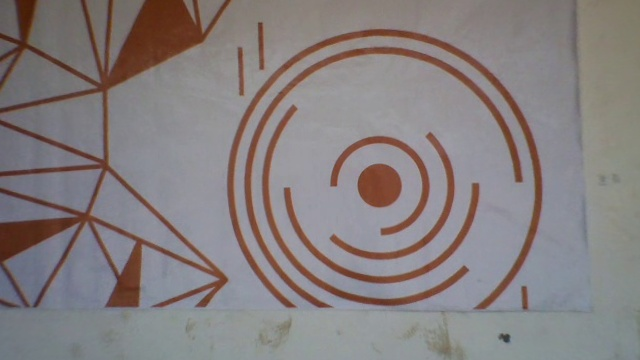
\includegraphics[width=0.48\textwidth]{images/left}
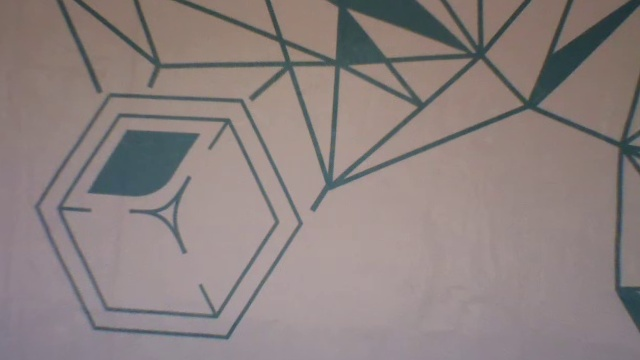
\includegraphics[width=0.48\textwidth]{images/right}
\caption[Example of super-panorama]{Candidate images for a super-panorama taken
from different depths. For context, see Fig.~\ref{fig:results}.  These images are
  `reference' images (spanning  tree center) of individual  mini-panoramas.}
\label{fig:exmaple}
\end{figure}

\textbf{Example:} Consider two images (shown in Fig.~\ref{fig:exmaple}) taken from the positions
(1.37, 0.85, 1.6), and (3.75, 0.98, 1.4).  As their depths are
different, we (virtually) move the second image by shrinking the
second image by a factor $\frac{1.4}{1.6}$, i.e., to 87\% of its
original size. With both images at the same depth (1.6m), the 
disparity of the second image is 
\begin{center}
$\text{disparity}_x = (3.75 - 1.37)f/1.6 = 839$\\
$\text{disparity}_y = (0.85 - 0.98)f/1.6 = -45$
\end{center}
where $f$ is focal length of the quadcopter camera in pixel units.

\subsection{Summary: Use of IMU}
The IMU data is used primarily for two purposes:
\begin{enumerate}
\item \textbf{Selection and ordering of images:} We use the IMU data
  to select representative images from the video and arrange them into
  rectangular grid according to the `spatial' neighborhood. It also
  disambiguates situations when multiple images that are spatially
  distant, but have similar, repeated features.

\item \textbf{Super-panorama:} Whenever there are no features in
  the overlap region of two images, we use the IMU data to find the
  relative position of one image w.r.t. second image as shown in the
  example. 
\end{enumerate}
\setlength{\tabcolsep}{2pt}
\section{Experiments and Results}
\label{sec:results}

All our experiments have been completed with the inexpensive consumer
quadcopter called a Parrot's AR Drone 2.0. The imagery acquired were
from actual graffiti painted on large walls as well as posters in an
exhibition.  We have used the ROS based ARDrone Autonomy
Driver to communicate with the drone. For the purpose of showing the
efficacy of our method, we also took a picture of the scene from a
distance with a smartphone camera to better understand the scene.

We have implemented our algorithm in C++ using the OpenCV library
(OpenCV 2.4.9). Experiments were performed on a PC with Intel Core i7
processor(@3.4GHz) and 8GB RAM.  
%The source code to produce
%interesting images from a video, and to generate the super-panorama,
%as well as the data sets used in this paper will be made publicly
%available after acceptance of the paper.

\subsection{Selecting Images}

In our first experiment, we wanted to ensure that the selection of
images done was comprehensive and useful.  We sent the drone to image 
an outdoor scene with no vacant space. This experiment was conducted
in an outdoor environment. We note here that there were approximately
3000 images in the raw video.  AutoStitch and Photoshop were unable to 
cope  when fed with this large number of frames.

One way to produce some sort of mosaic was to simply reduce the amount
of data given to AutoStitch.  Figure~\ref{fig:sac3}(a) shows uniformly
(time) sampled images from the video.  When these sampled images are
given to AutoStitch or to Adobe Photoshop, we find
(Figure~\ref{fig:sac3}(b)) that these programs are able to produce
some output, but the results are not satisfactory.

Instead of feeding time-sampled images, we ran our albumization
algorithm (as explained in Section~\ref{sec:selection}) on the video
which resulted in $N = 5$ images.  Though the number of input images
in the video is large, the total distance covered by the quadcopter in
this duration (of around 90 seconds) is small; thus the
number of distinct images returned by the algorithm shows a dramatic
reduction. Figure~\ref{fig:sac3}(c) shows examples of selected images.
Many of the images are similar to the time sampled version; however,
the occasional differences are enough to make AutoStitch work. The
results are shown in Figure~\ref{fig:sac3}(d).


\begin{figure}[hb!]
\centering
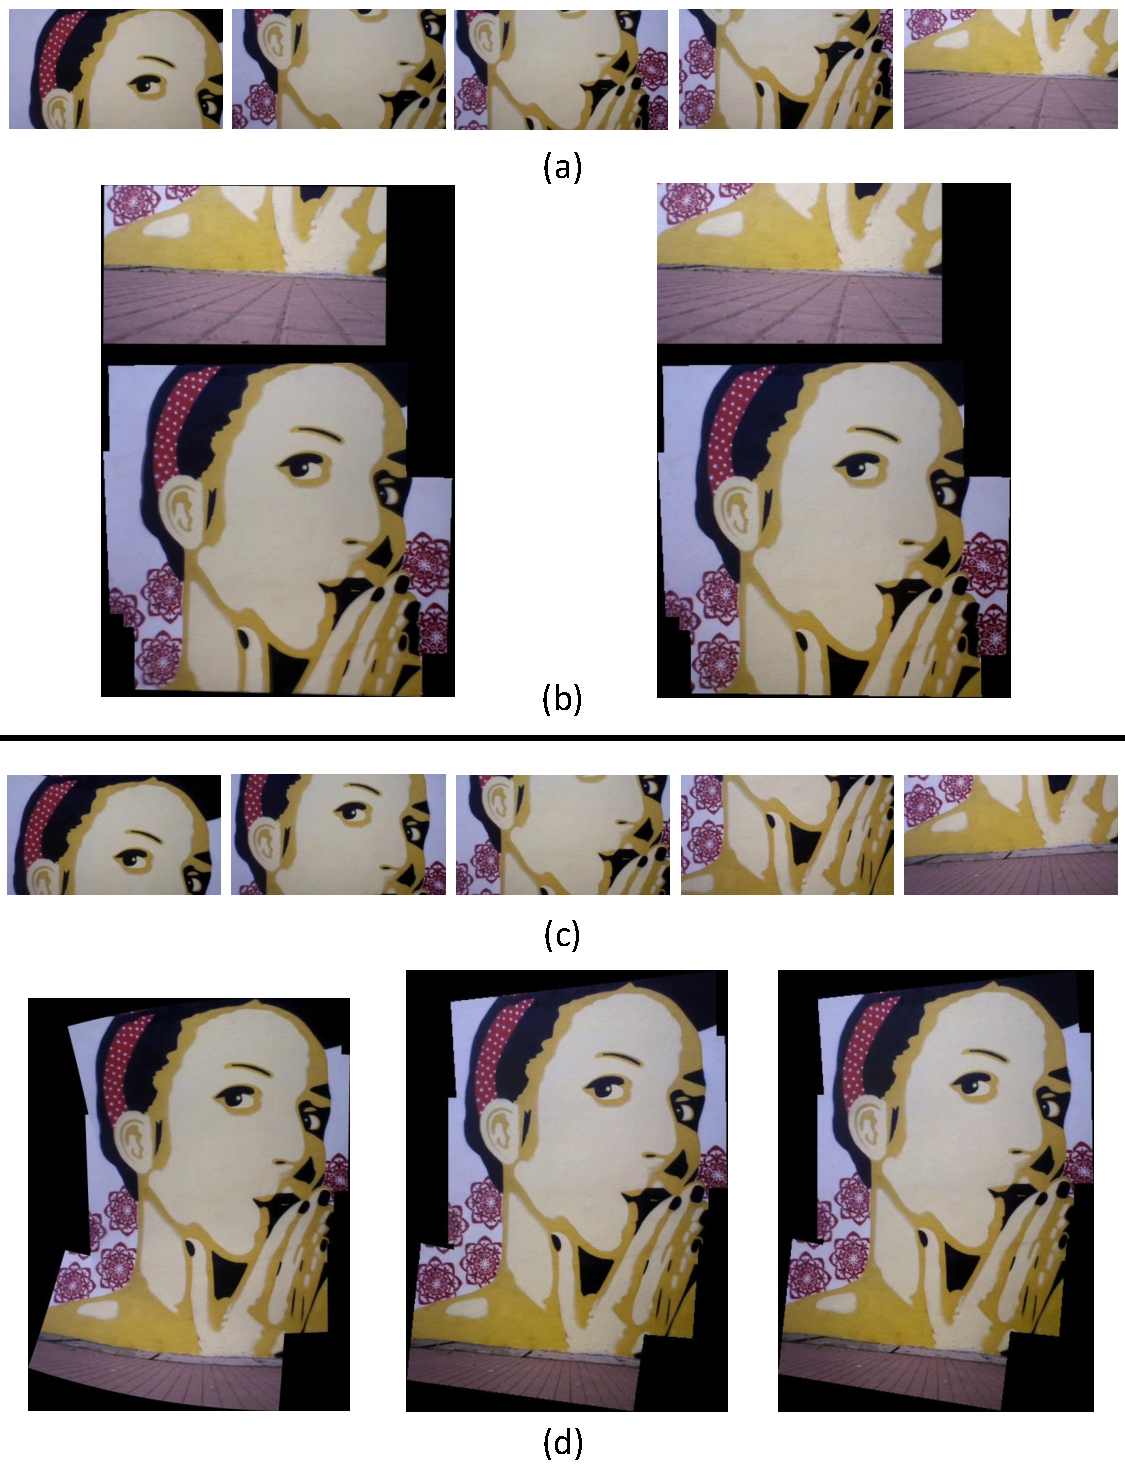
\includegraphics[width=0.87\linewidth]{figures/vacantSpaces/ValidationResult}
\caption[Validation Result: Lady]{ (a) Uniformly sampled images from an outdoor
video expedition.  (b) Output of the state of the art photo stitchers
  (left:AutoStitch, right:Adobe Photoshop CS6) on uniformly time
  sampled images.  As time sampled images do not guarantee coverage of
  the scene, the panorama is broken. The top portions do not belong at
  the right place (see (d)) (c) Salient image selection from the set of
  approximately 3000 images using positional information. (d) When
  salient images are given to AutoStitch (left) and Photoshop (middle),
  we can create a panoramic mosaic (since there are no vacant
  spaces). We also show the result from our stitching algorithm
  (bottom right).}
\label{fig:sac3}
\end{figure}

In summary, this experiment provides evidence to show that (a) our
albumization algorithm is reasonable and (b) our stitching
results are comparable to that of AutoStitch for the kind of scenes
considered.

\subsection{Indoor Imagery with Vacant Spaces}

Our next selection of experiments were conducted in an indoor
environment.  

The input stream had about 4300
images. The selection algorithm (Section~\ref{sec:selection}) pruned the video
into $N=5$ images. A sample of the selected images are seen in Figure~\ref{fig:vacantTeaser}.

There were two disconnected components in the resulting graph.
AutoStitch was unable to produce any reasonable output as seen in
Figure~\ref{fig:vacantTeaser}.  The scene, captured from a distance is also
shown.  One can see a better orthographic view of the posters.

\textbf{Cars:}
In an another experiment, the input stream had about 9000 input
images.  The selection algorithm (Section~\ref{sec:selection}) pruned
the video into $N=13$ images. A sample of the selected images are seen
in Figure~\ref{fig:indoor_results}(a).  The scene as captured by a
smartphone can also be seen, as well as the outputs of the state of
the art stitchers. Note that AutoStitch is only able to stitch the
upper half of the scene.  Our result
Figure~\ref{fig:indoor_results}(e) clearly stands out in comparison.

\begin{figure}
\centering
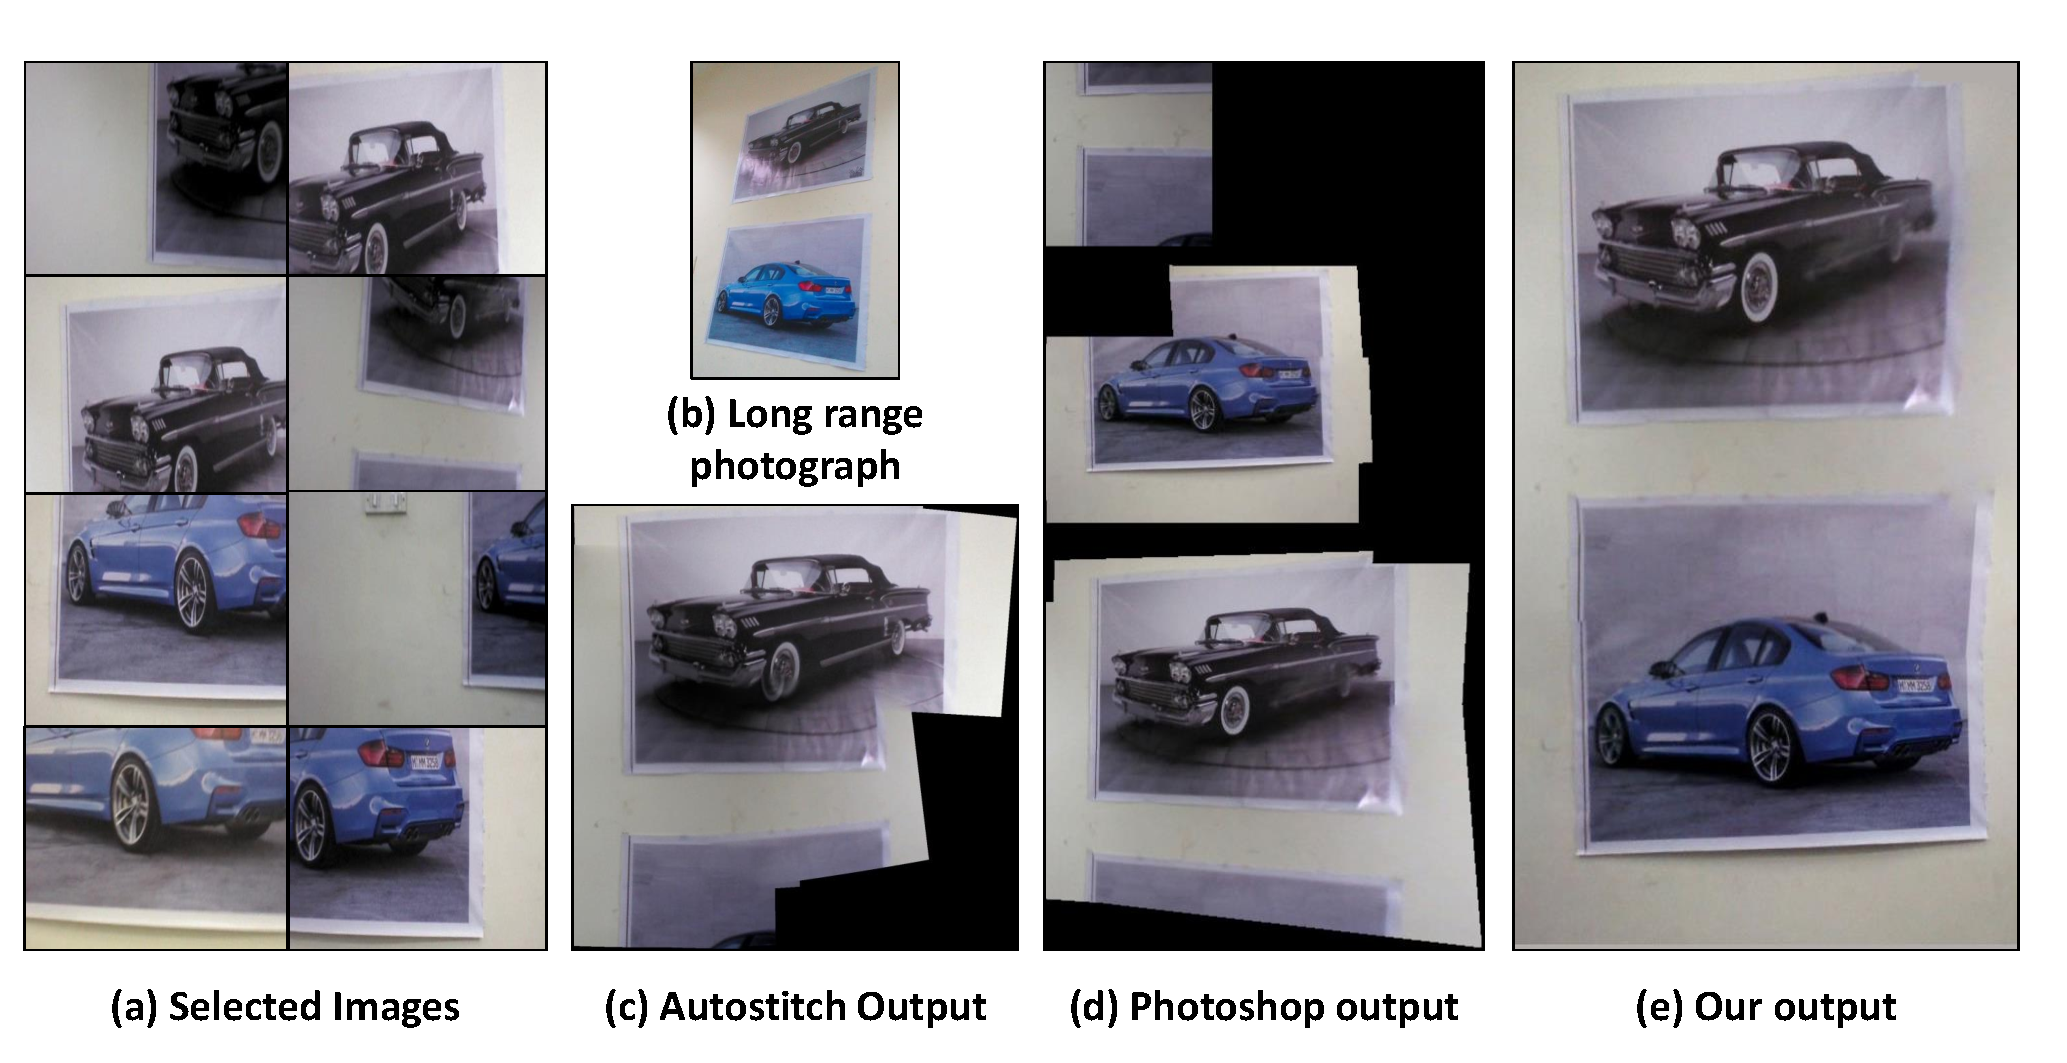
\includegraphics[width=\linewidth]{figures/vacantSpaces/indoor_results}
\caption[Result: Cars]{ (a) Pruned images from the quadcopter video using our
  saliency algorithm of (b) an indoor scene. This long range photograph
  has been captured separately by a smartphone camera only for
  context. Notice a significant vacant space in the imagery.  (c)
  Output of AutoStitch -- only the upper half of the scene is output.
  (d) Output of Adobe Photoshop CS6 -- the vacant space posed a problem to the
  feature matching algorithm, so instead of a mosaic, individual
  pieces were output as mini-panoramas (e) Our output on the selected
  images. We are able to present the scene in high fidelity in an
  orthographic view.}
\label{fig:indoor_results}
\end{figure}

\textbf{Aircrafts 1:} The input stream had about 9100 images. The selection
algorithm pruned the video into $N=14$ images. The scene as captured by a
smartphone can also be seen in Figure~\ref{fig:aircrafts1}(b). A sample of the
selected images are seen in Figure~\ref{fig:aircrafts1}(a).
Figure~\ref{fig:aircrafts1}(c,d,e) shows the comparison of outputs of state of
the art stitchers with the output of our algorithm. As there are vacant spaces,
AutoStitch~\cite{autostitch} is able to join only top part of the scene, while
Photoshop~\cite{photoshop} is showing two disconnected components.
In contrast, since we use positional data, our output is an acceptable mosaic,
and shows an orthographic view.

\begin{figure*}[h!]
	\centering
	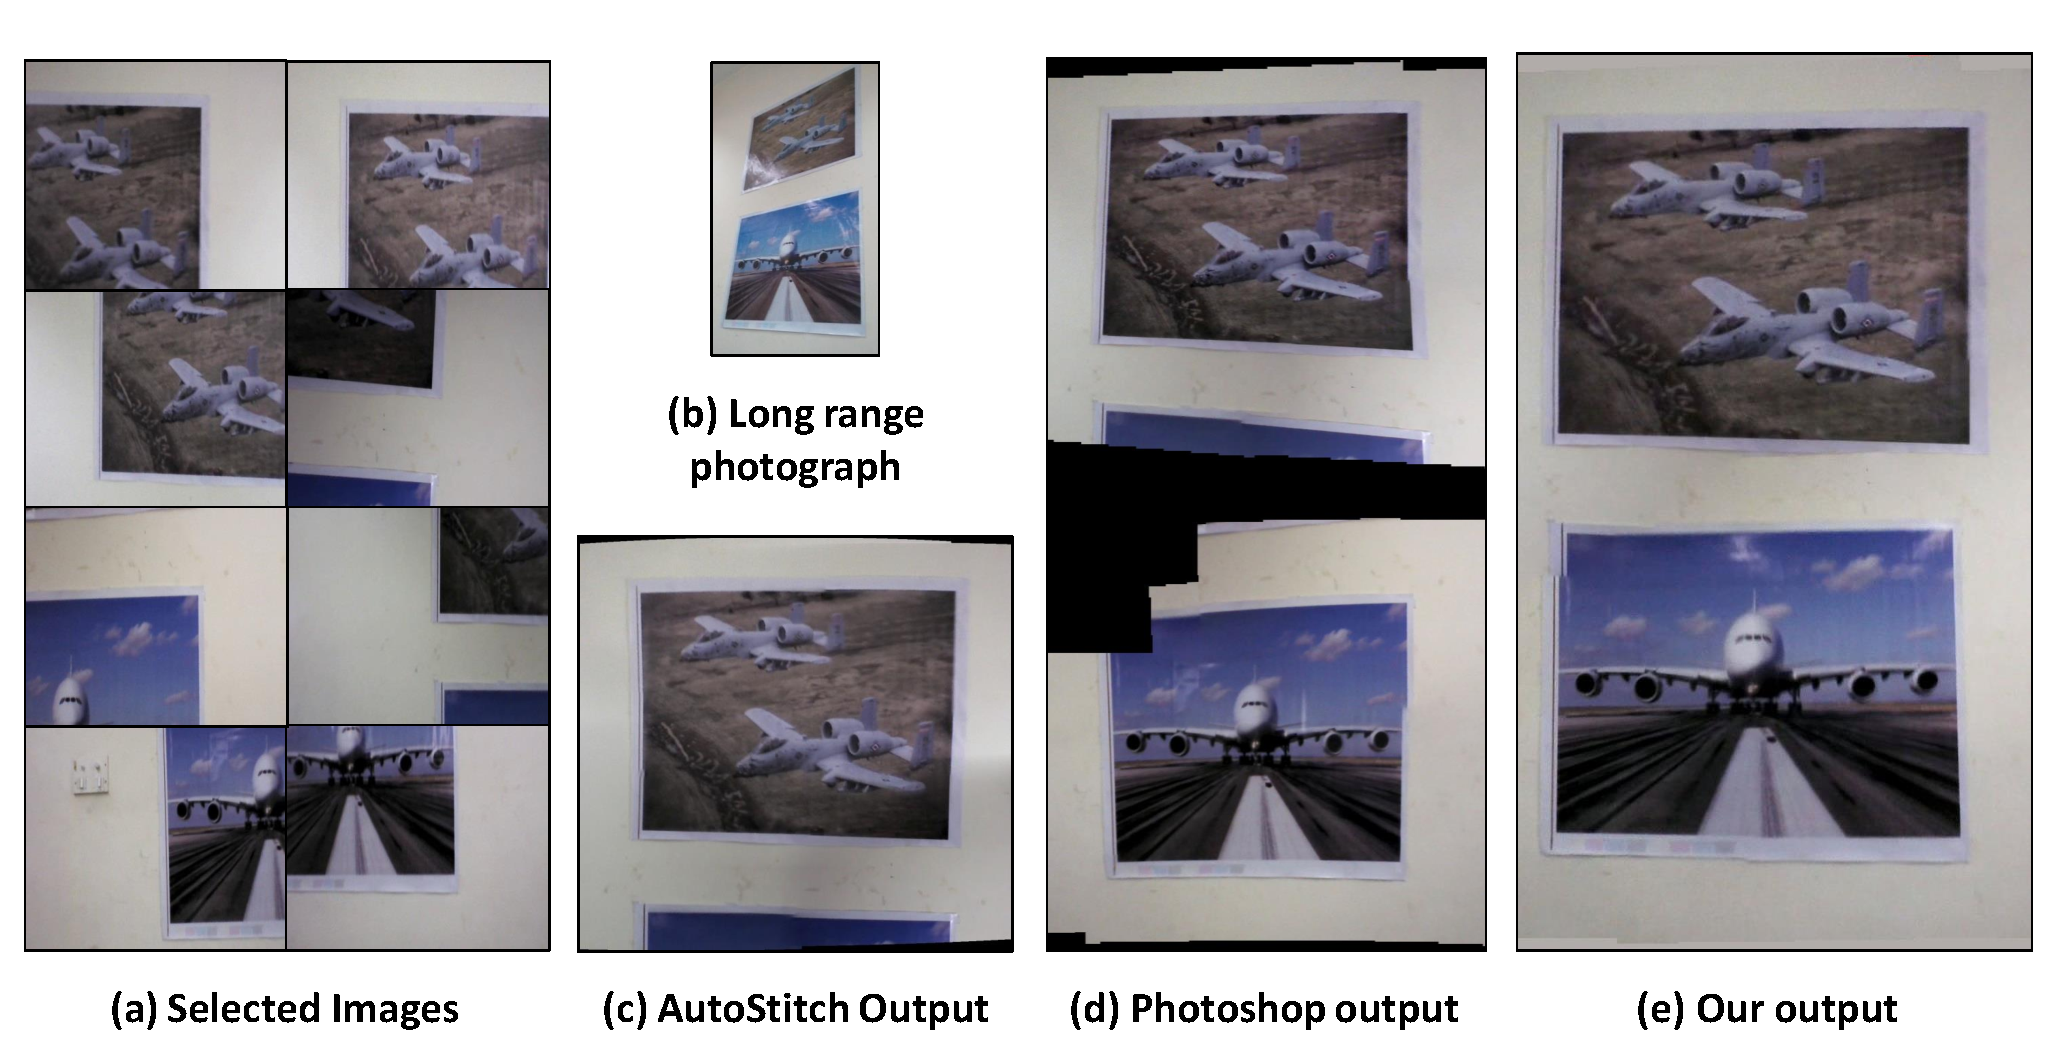
\includegraphics[width=\linewidth]{figures/vacantSpaces/aircrafts1}
	\caption[Result: Aircrafts]{(a) Pruned images from the quadcopter video using
	our saliency algorithm of (b) an indoor scene. This long range photograph has been captured separately by a smartphone camera only for context. Notice a significant vacant
space in the imagery. (c) Output of AutoStitch - only the upper half of the scene is output. (d) Output of Adobe Photoshop CS6 - 
the vacant space posed a problem to the feature matching algorithm, so instead of a mosaic, individual pieces were output as mini-panoramas (e) Our output on the
selected images. We are able to present the scene in high fidelity in an orthographic view.}
	\label{fig:aircrafts1}
\end{figure*}

\subsection{Outdoor Imagery with Vacant Spaces}

\begin{figure}[h!]
\centering
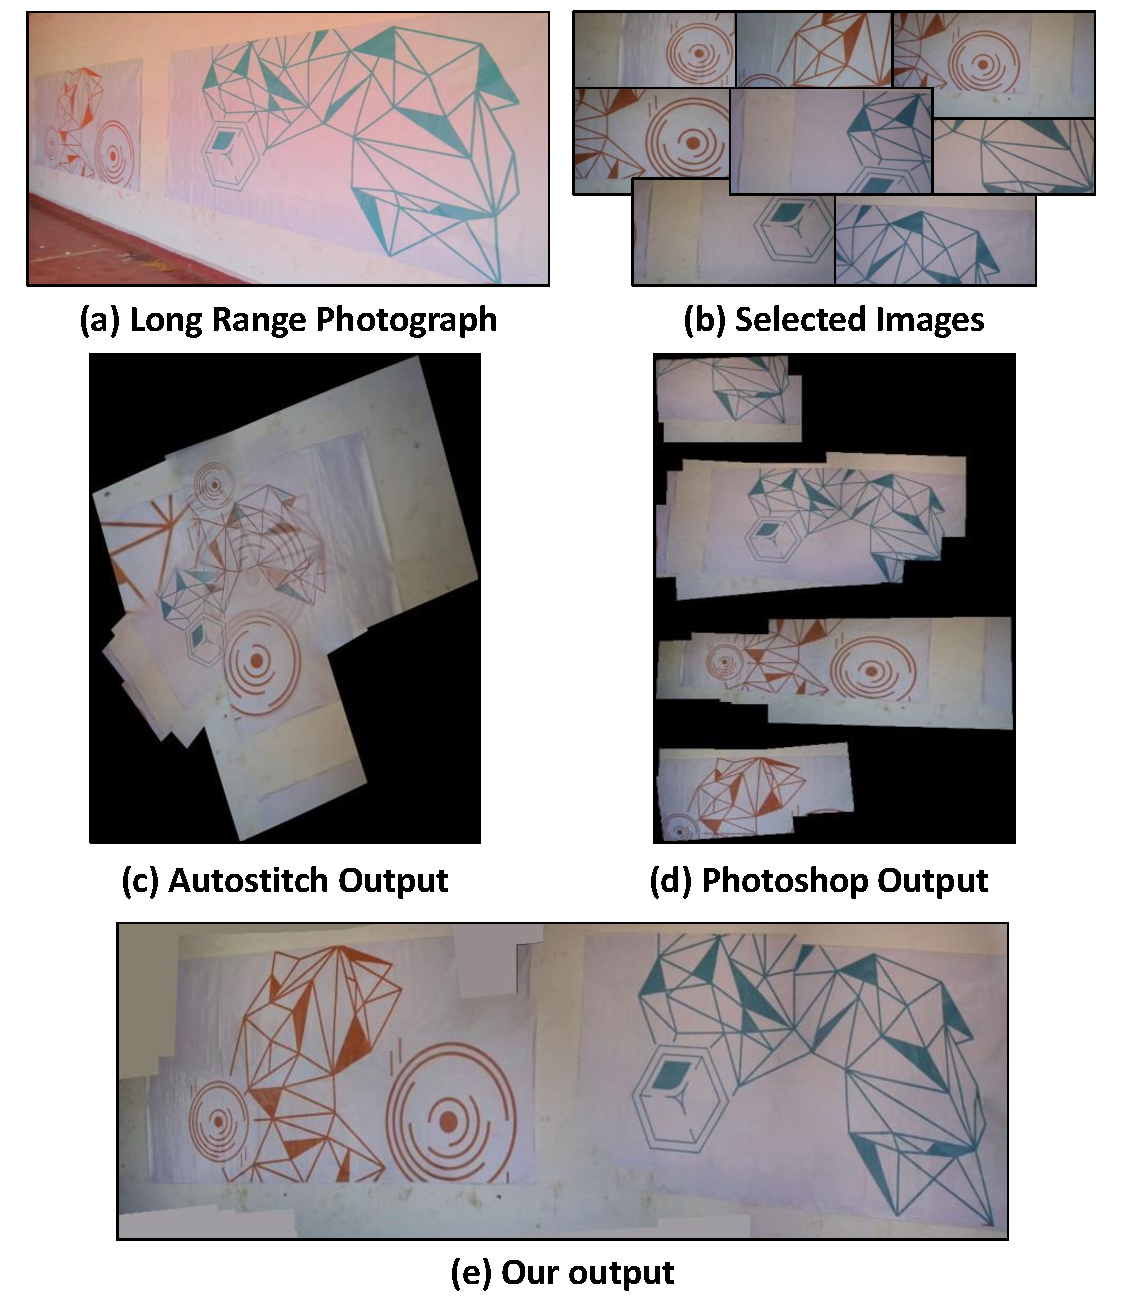
\includegraphics[width=\linewidth]{figures/vacantSpaces/orange_blue}
\caption[Result: Outdoor Exhibition]{(a) An outdoor scene captured by a standard
camera in an exhibition. The approach to the area is normally cordoned off and one
  needs permission to get a quadcopter to take the picture.  Notice a
  significant gap between the two posters.  (b) Pruned images from the
  quadcopter video using our saliency algorithm. (c) Output of
  AutoStitch on the selected images. The mosaic is not reasonable
  presumably because of the confusion in features. (d) Output of Adobe
  Photoshop CS6 on the selected images. The vacant space posed a
  problem to the feature matching algorithm, so instead of a mosaic,
  individual pieces were output as mini-panoramas (e) Our output on
  the selected images. We are able to join two posters (separated by
  vacant space) using the IMU data.}
\label{fig:results}
\end{figure}

Our next set of experiments were conducted in an outdoor
environment. The input stream had about 12000 images. The selection
algorithm pruned the video into $N=30$ images. A sample of the
selected images are seen in Figure~\ref{fig:results}(a).  The scene as
captured by a smartphone can be seen in Figure~\ref{fig:results}(b).
Figures~\ref{fig:results}(c), (d) and (e) shows the comparison of outputs of
state of the art stitchers with the output of our algorithm. Note that
AutoStitch is getting confused by too many matching features. 
Please see supplementary material for results on other indoor as well as outdoor datasets.

Figure \ref{fig:results2} shows comparison of outputs of state of the art
stitchers with output of our algorithm on another dataset.

\begin{figure}[h!]
\centering
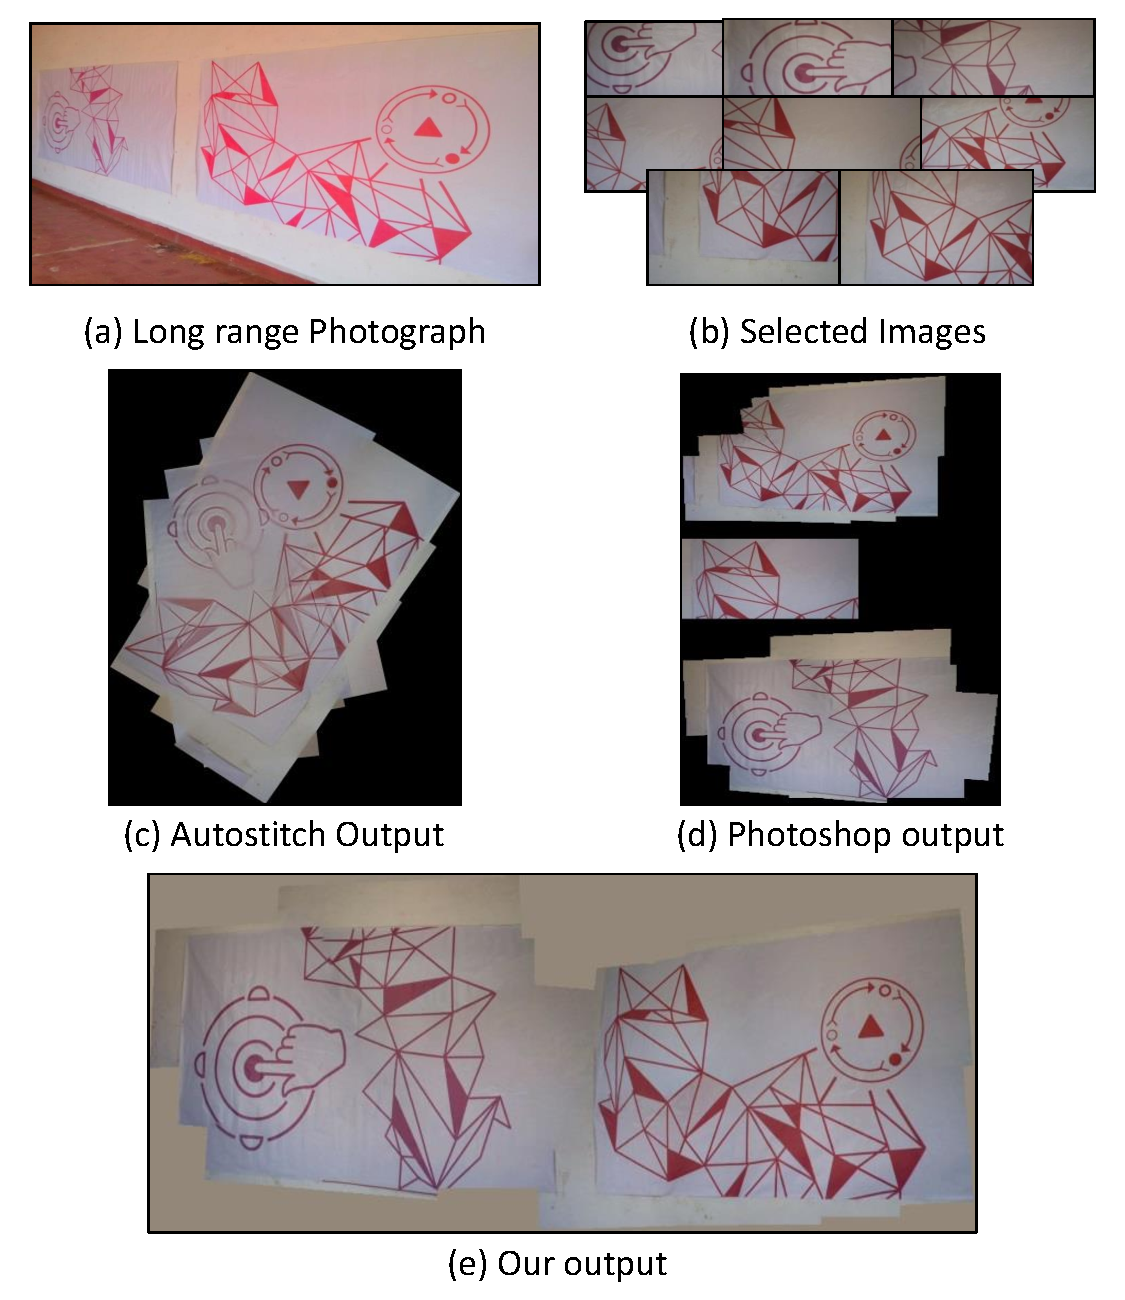
\includegraphics[width=\linewidth]{figures/vacantSpaces/Purple_red} 
\caption[Result: Outdoor
Exhibition 2]{(a) Another outdoor
scene captured by a standard camera in an exhibition. The approach to the area is normally cordoned off and one
  needs permission to get a quadcopter to take the picture.  Notice a
  significant gap between the two posters.  (b) Pruned images from the
  quadcopter video using our saliency algorithm. (c) Output of
  AutoStitch on the selected images. The mosaic is not reasonable
  presumably because of the confusion in features. (d) Output of Adobe
  Photoshop CS6 on the selected images. The vacant space posed a
  problem to the feature matching algorithm, so instead of a mosaic,
  individual pieces were output as mini-panoramas (e) Our output on
  the selected images. We are able to join two posters (separated by
  vacant space) using IMU data.}
\label{fig:results2}
\end{figure}


\subsection{Analysis}

The performance of our algorithm as a function of the scene, as well
comparison with other software is summarized in
Table~\ref{tbl:results}.  It can be seen that, whenever there is
vacant spaces between adjacent images, AutoStitch produces only
one component, presumably the largest.  Adobe Photoshop outputs all disconnected
components. Sometimes due to the lack of spatial proximity
information, the resulting images (or components) are disconnected instead of being 
mosaiced (unlike AutoStitch). In contrast, in all cases, our algorithm
successfully uses proximity information which results in a reduced number of mini-panoramas. 

As expected the number of selected images in our saliency algorithm
varies based on environment considerations (outdoor/indoor), the
average depth from the scene, and the total scene area.
 
\begin{table*}
\scriptsize

\newcolumntype{C}{ >{\centering\arraybackslash} m{1.1cm} }
\newcolumntype{D}{ >{\centering\arraybackslash} m{1.5cm} }

\begin{tabular}{|C|C|C|C|D|D|D|m{6.5cm}|}
\hline
Dataset 
& Number of Images in video 
& Approx. planar area covered
& Number of selected images 
& AutoStitch: \# Components 
& Photoshop: \# Components
& Our algorithm: \#mini- panoramas
& \multicolumn{1}{p{6.5cm}|}{\centering Remarks}\\
\hline

\hyperref[fig:sac3]{Lady} & 3000 & 60 sqft. & 5 & 1 & 1 & 1 & As there are enough features
in the intersection of selected images, AutoStitch, Photoshop as well
as our algorithm produces the  panorama correctly.\\\hline
%Spray Woman} & 9000 & 70 sqft. & 15 & 1 &
%1 & 1 & As there are enough features in the intersection of selected images,
%AutoStitch, Photoshop as well as our algorithm gives full panorama
%correctly. As this scene was captured nearer from the plane than
%earlier, we need to select more images than earlier dataset.\\\hline 

\hyperref[fig:vacantTeaser]{Indoor exhibition} & 4300 & 40 sqft. & 5 &
1 & 2 & 2 & As there is vacant space between the two posters,
AutoStitch produces only one panoramic image. Photoshop outputs two
posters as two disconnected components; these correspond to our mini-panoramas.
\\\hline 

\hyperref[fig:indoor_results]{Cars} & 9000 & 60 sqft. & 13 & 1 & 3 & 3 &
As there is vacant space between the two visuals, AutoStitch produces
only one panoramic image, the black vehicle.  In the case of
Photoshop, two of the three disconnected 
components represents two partial visuals, while the third component is
the intersection  between the two cars -- this portion contains featureless
space.\\\hline

\hyperref[fig:results]{Outdoor exhibition} & 12000 & 80 sqft. &
30 & 1 & 4 & 2 &  AutoStitch is confused by the replicated features in
the two posters which are sometimes proximal and sometimes
geographically distant.  A single panorama is produced, but the output
is incorrect. We use the IMU data
for arranging the images in spatial neighborhood; we have fewer
mini-panoramas.  Photoshop is not able to produce a super-panorama and
the number of disconnected components in Photoshop's output is larger
than the number of mini-panoramas.\\\hline  
\end{tabular}
\caption{Quantitative summary of  results.}
\label{tbl:results}
\end{table*}



\section{Concluding remarks}

In this chapter, we have described a method of imaging large scenes
using a quadcopter enabling close orthographic views. We also defined
a new problem, that of computing a mosaic of a planar scene with
vacant spaces.  Vacant space relates to images in an input stream
where there are not enough features for traditional mosaicing
algorithms to estimate geometric warps to align the images.

Our solution to this problem is to use a quadcopter which
is capable of taking pictures.  The quadcopter has an inertial
measurement unit that is capable of outputting approximate
positions. Using this positional information, our algorithm selects an
``interesting'' subset of the video imagery.  This subset consists of
pictures taken with a moving camera; we reduce the resulting
problem of computing a mosaic to the stereo problem.  Our
method works on both indoor and outdoor scenes.

Controlling a consumer-focused inexpensive quadcopter can be
problematic; for instance the quadcopter could have severe yaw and
roll.  We need a robust algorithm for autonmous navigation of quadcotper.
We will discuss vision based algorithms to control such quadcopters autonomously
in next chapter. We extend our work of mosacing scene on single planar
surface to scene spread over multiple planar surface.